\section{Architectural design}

\subsection{Overview}
	\subsubsection{Context viewpoint}
	
		\begin{figure}[h]
			\centering
			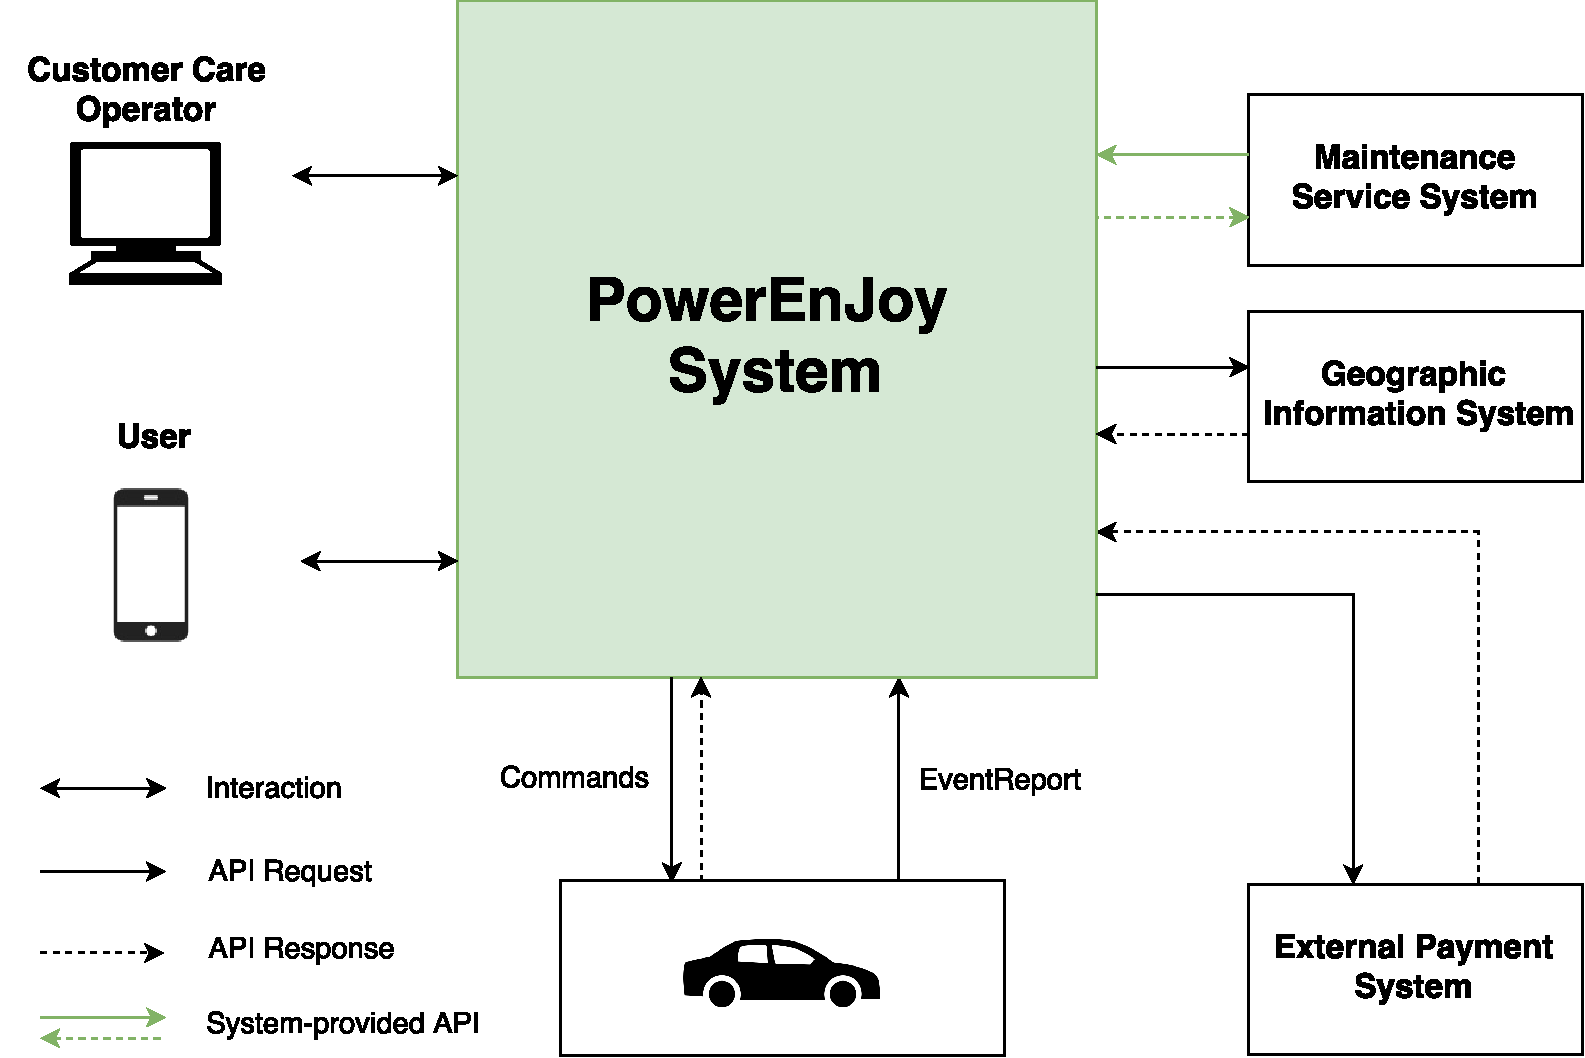
\includegraphics[width=\linewidth]{contextViewPoint}
			\caption{
				\label{fig:contextViewPoint} 
				Context viewpoint
			}
		\end{figure}
		
		We need to design a system which allows communications with many agents such as cars, users, external systems, etc.
		Moreover we recognize that in most of the interactions the system is providing a service to agents so, after taking in consideration different alternatives, we decided to use a client-server architectural approach.

		\begin{figure}[h]
			\centering
			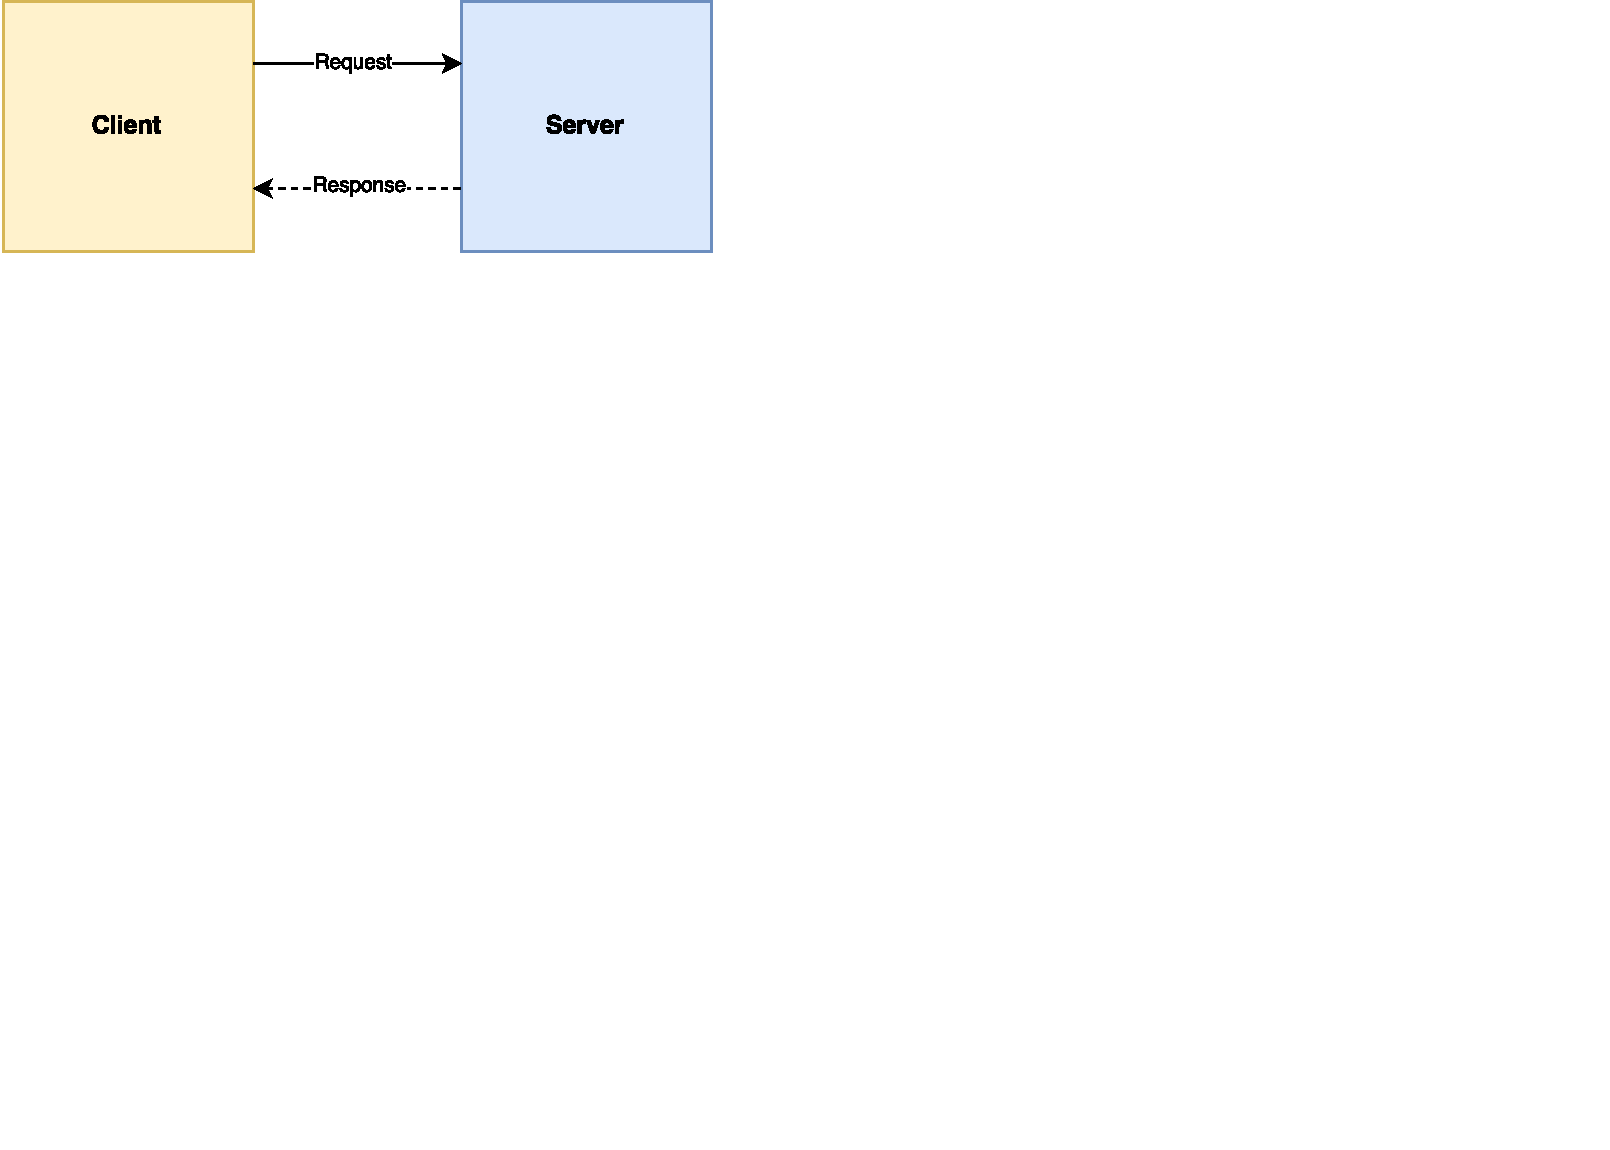
\includegraphics[width=0.5\linewidth]{ClientServer}
			\caption{
				\label{fig:ClientServer} 
				Client Server architecture
			}
		\end{figure}
		
		Cars offer to the system a set of primitives which allow it to interact with them: in this case it is clear that cars are providing the system services, so they can be identified as servers while the system acts as a client; on the other end the notification functionality offered by cars clearly yields to an event-based approach due to the asynchronous nature of such interactions, this led us to use a publish-subscribe paradigm for these specific interactions.
		\clearpage
		
		
		
	\subsubsection{Composition viewpoint}
	
		\begin{figure}[h]
			\centering
			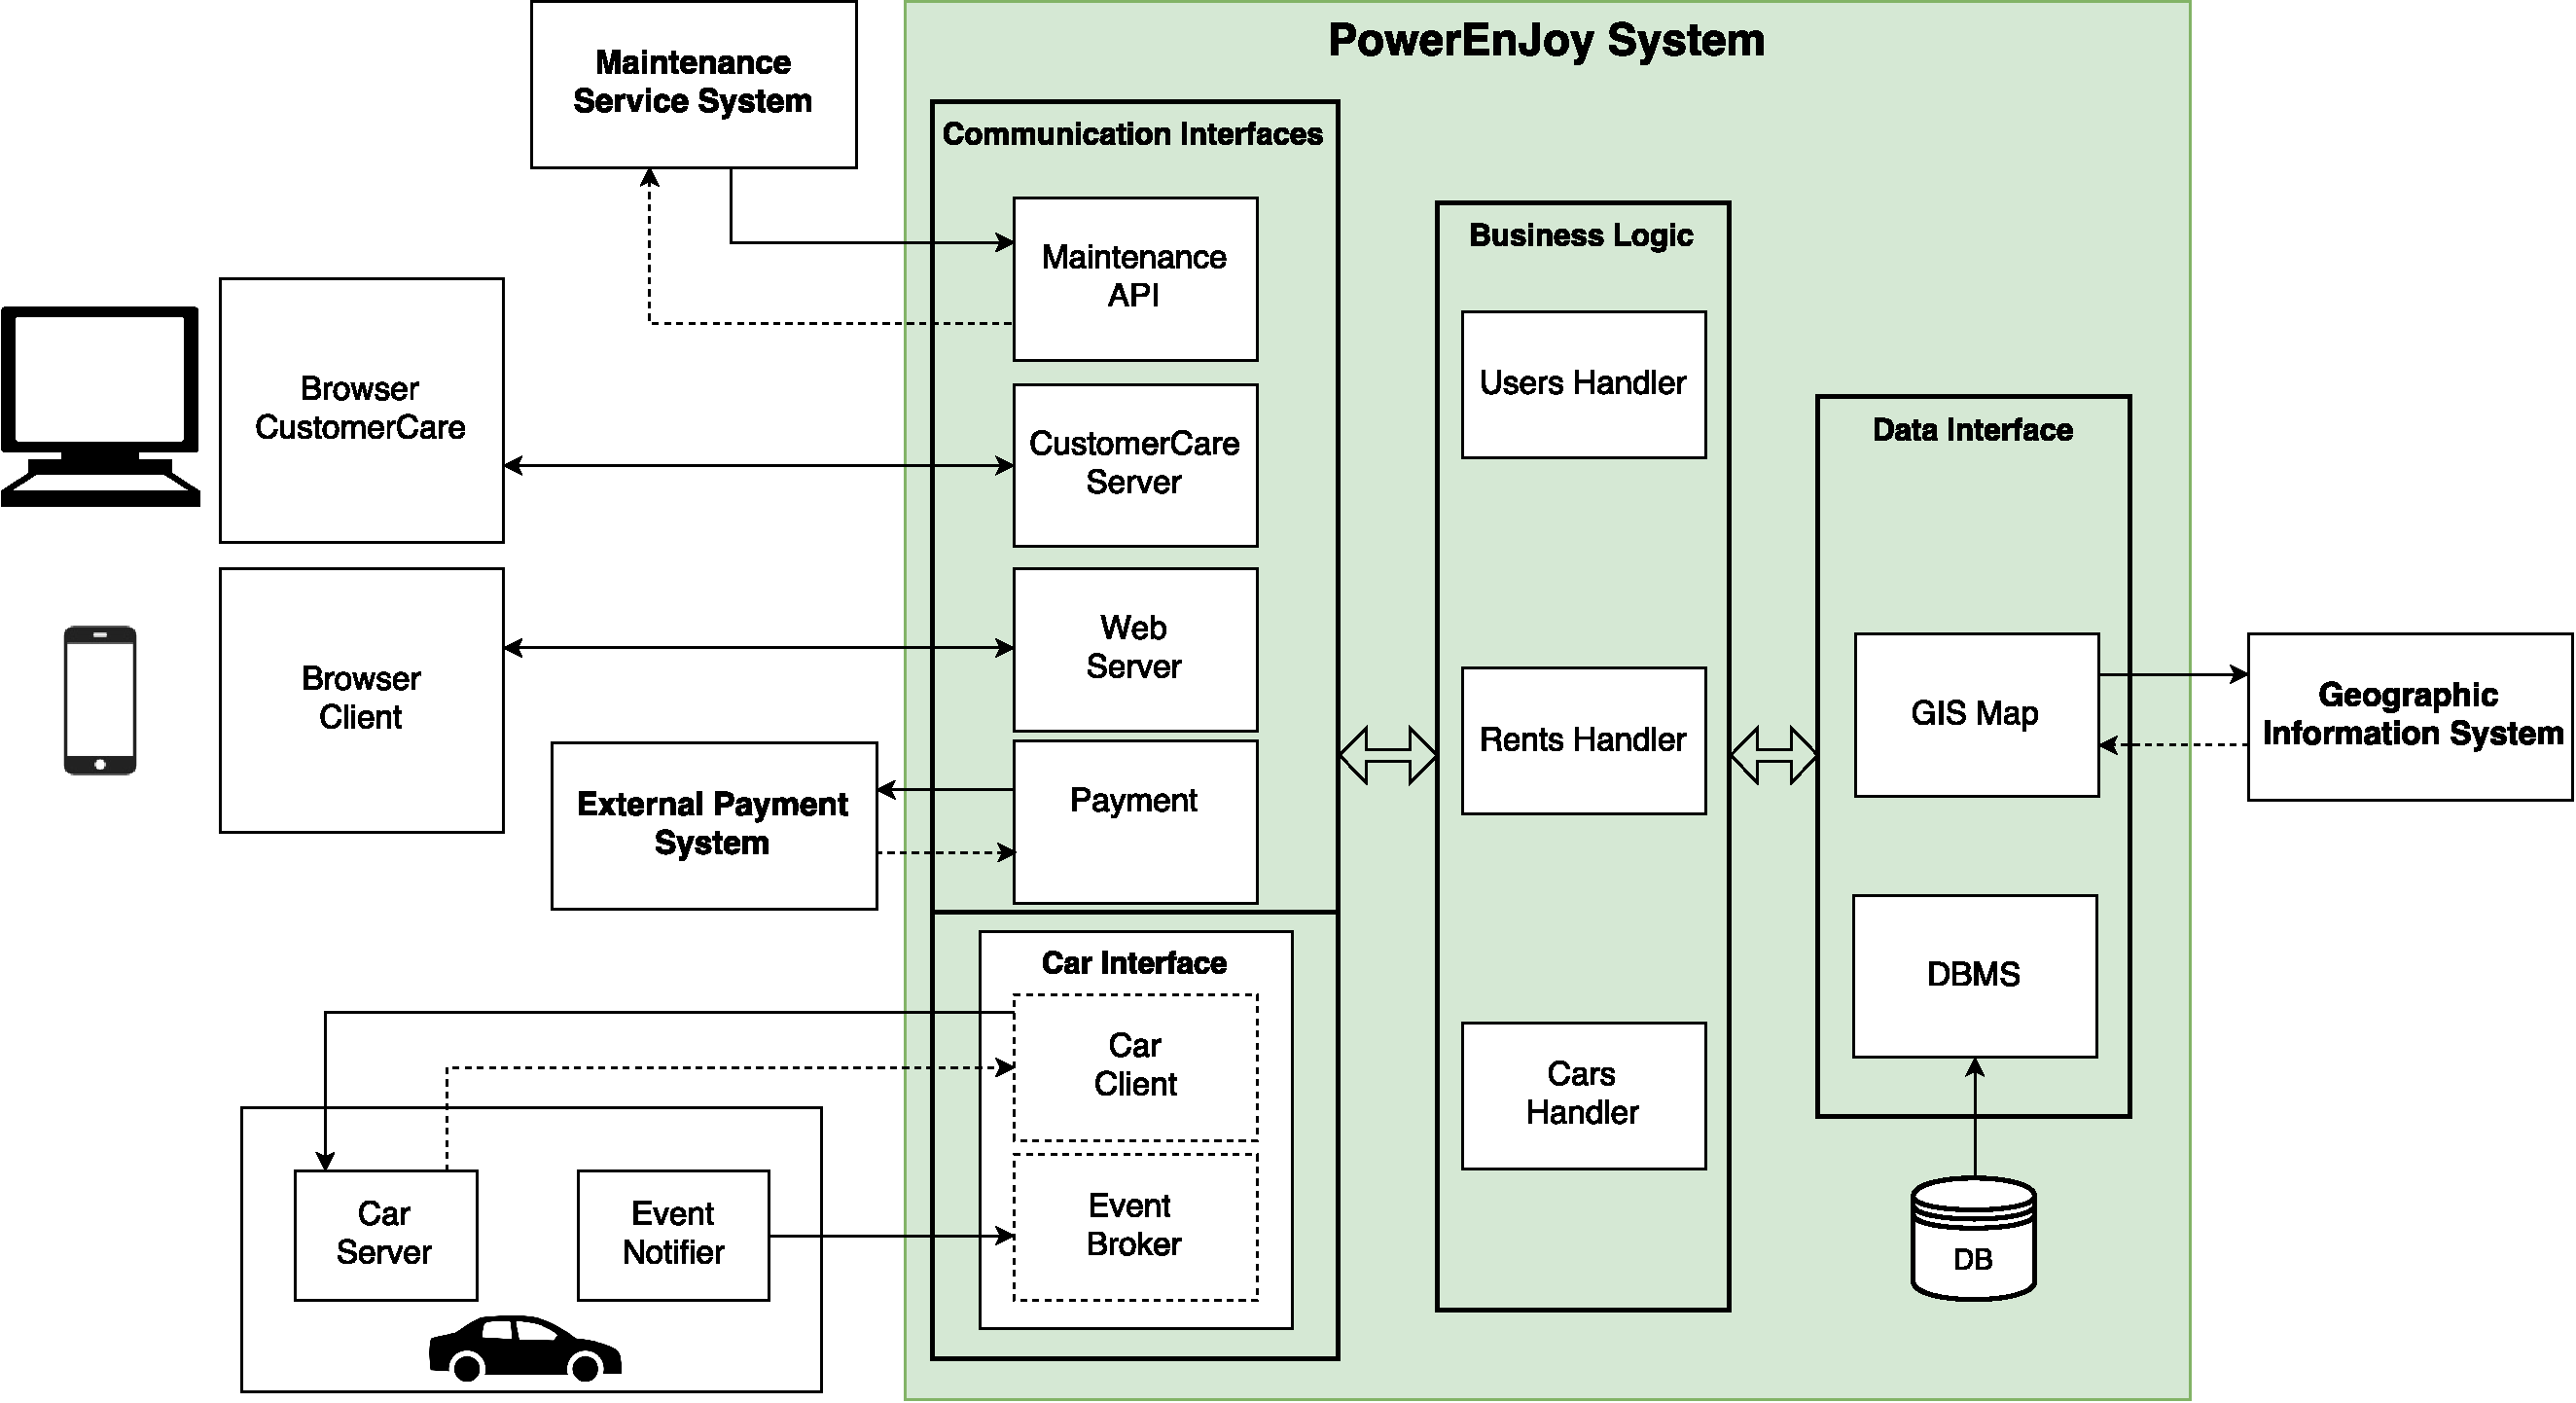
\includegraphics[width=\linewidth]{ComponentOverview}
			\caption{
				\label{fig:compositionViewPoint} 
				Composition viewpoint
			}
		\end{figure}
		
		Going deeper in the analysis of our system composition, we are able to identify some of the modules that will be required in order to provide the functionalities specified in the Requirement Analysis and Specification Document. 
		\paragraph{Communication Interfaces}
			Since our system interacts with many external agents, it needs to have different \emph{Communication Interfaces} in order to communicate with them. 
		\begin{itemize}
			\item An API is needed to provide \emph{Maintenance Service System} the information it needs to work with us
			\item A software module is needed to provide the \emph{Customer Care} the functionalitities it needs
			\item A web server is needed in order to communicate with the users
			\item An internal payment software module will deal with the communication with the \emph{External Payment System} 
			\item A set of modules will manage the communications between the cars and the system: a module to call primitives on cars through the provided API and another one to observe events triggered by the car
		\end{itemize}
		\paragraph{Business Logic}
			The actual application logic of our system needs to manage the users information, the rents and the cars information; for each of these purposes several software modules are necessary; they will use communication interfaces to communicate with the agents and they will be able to retrieve data from the data interfaces.
		\paragraph{Data Interface}
			Our system needs a way to access and store the data it produces or retrieves from external resources, that is why \emph{Data Interface} modules are needed. These modules allows interaction between the \emph{Business Logic} modules and the System Databases; moreover they provide an interface to communicate with the GIS in order to allow the \emph{Business Logic} modules to access its functionalities.



\subsection{Component view}
\begin{figure}[h]
	\centering
	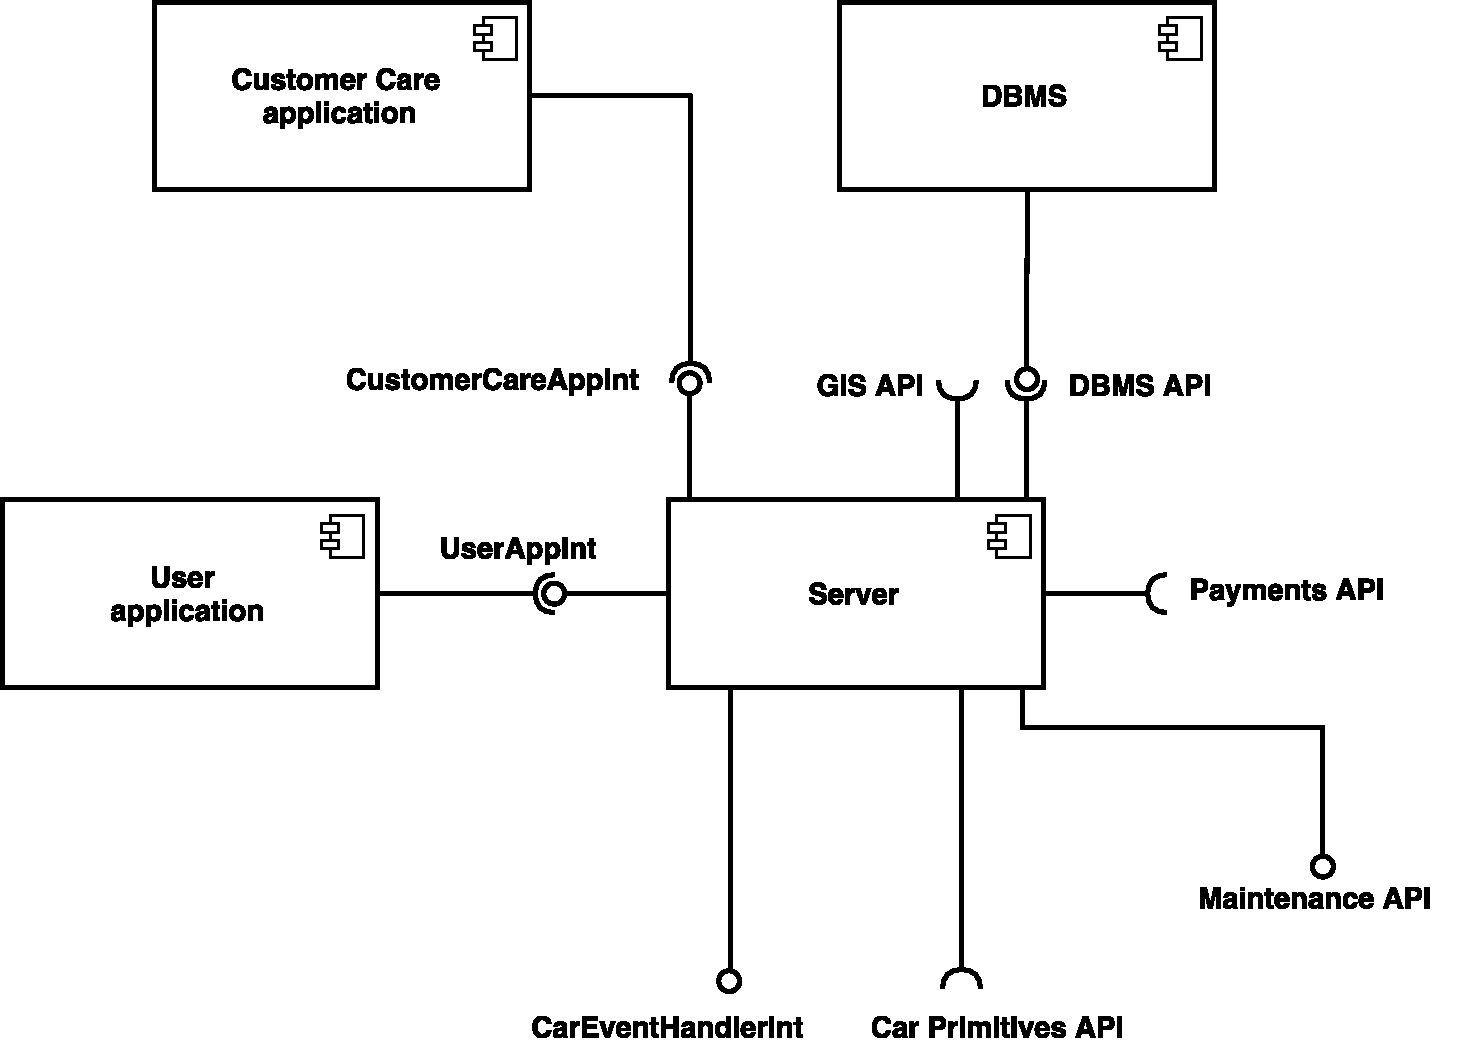
\includegraphics[width=\linewidth]{highLevelComponents}
	\caption{
		\label{fig:highLevelComponents} 
		High-level components
	}
\end{figure}
Considering all the previous graphs, we have identified in \autoref{fig:highLevelComponents} the following high level components, interfaces and mapping of the functionality defined in the RASD:
\begin{itemize}

	\item User application
	\begin{itemize}
		\item Register
		\item Login
		\item View the map with the position of
		\begin{itemize}
			\item himself
			\item safe areas
			\item available cars (with their battery level)
			\item charging stations
		\end{itemize}
		\item Reserve a car
		\item View customer care contacts
		\item Unlock the reserved car
		\item View and edit personal information
		\item View rents and payments history
	\end{itemize}
	
	\item Customer Care application
	\begin{itemize}
		\item View each user profile, including personal information, progress of the current rent, rent and payments history
		\item Mark and unmark users as banned
		\item Mark cars as Not Available
	\end{itemize}
	
	\item DBMS
	\begin{itemize}
		\item Store and retrieve data
	\end{itemize}	
	
	\item GIS API
	\begin{itemize}
		\item Get a map which will be populated with markers
	\end{itemize}
	
	\item Payments API
	\begin{itemize}
		\item Execute payment transactions
	\end{itemize}
	
	\item Maintenance API
	\begin{itemize}
		\item Expose the list of the cars tagged as Not Available with their GPS position and a brief description of the problem
		\item Tag Not Available cars as Available
	\end{itemize}
	
	\item Car Primitives API
	\begin{itemize}
		\item Call car embedded system's primitives
	\end{itemize}
	
	\item Car Event Handler Interface
	\begin{itemize}
		\item Triggered by an event notification from cars
	\end{itemize}
\end{itemize}
\clearpage

\subsubsection{DB component}
\paragraph{ER model}In \autoref{fig:ERModel} is represented the ER model of the system's database.

\begin{figure}[h!]
	\centering
	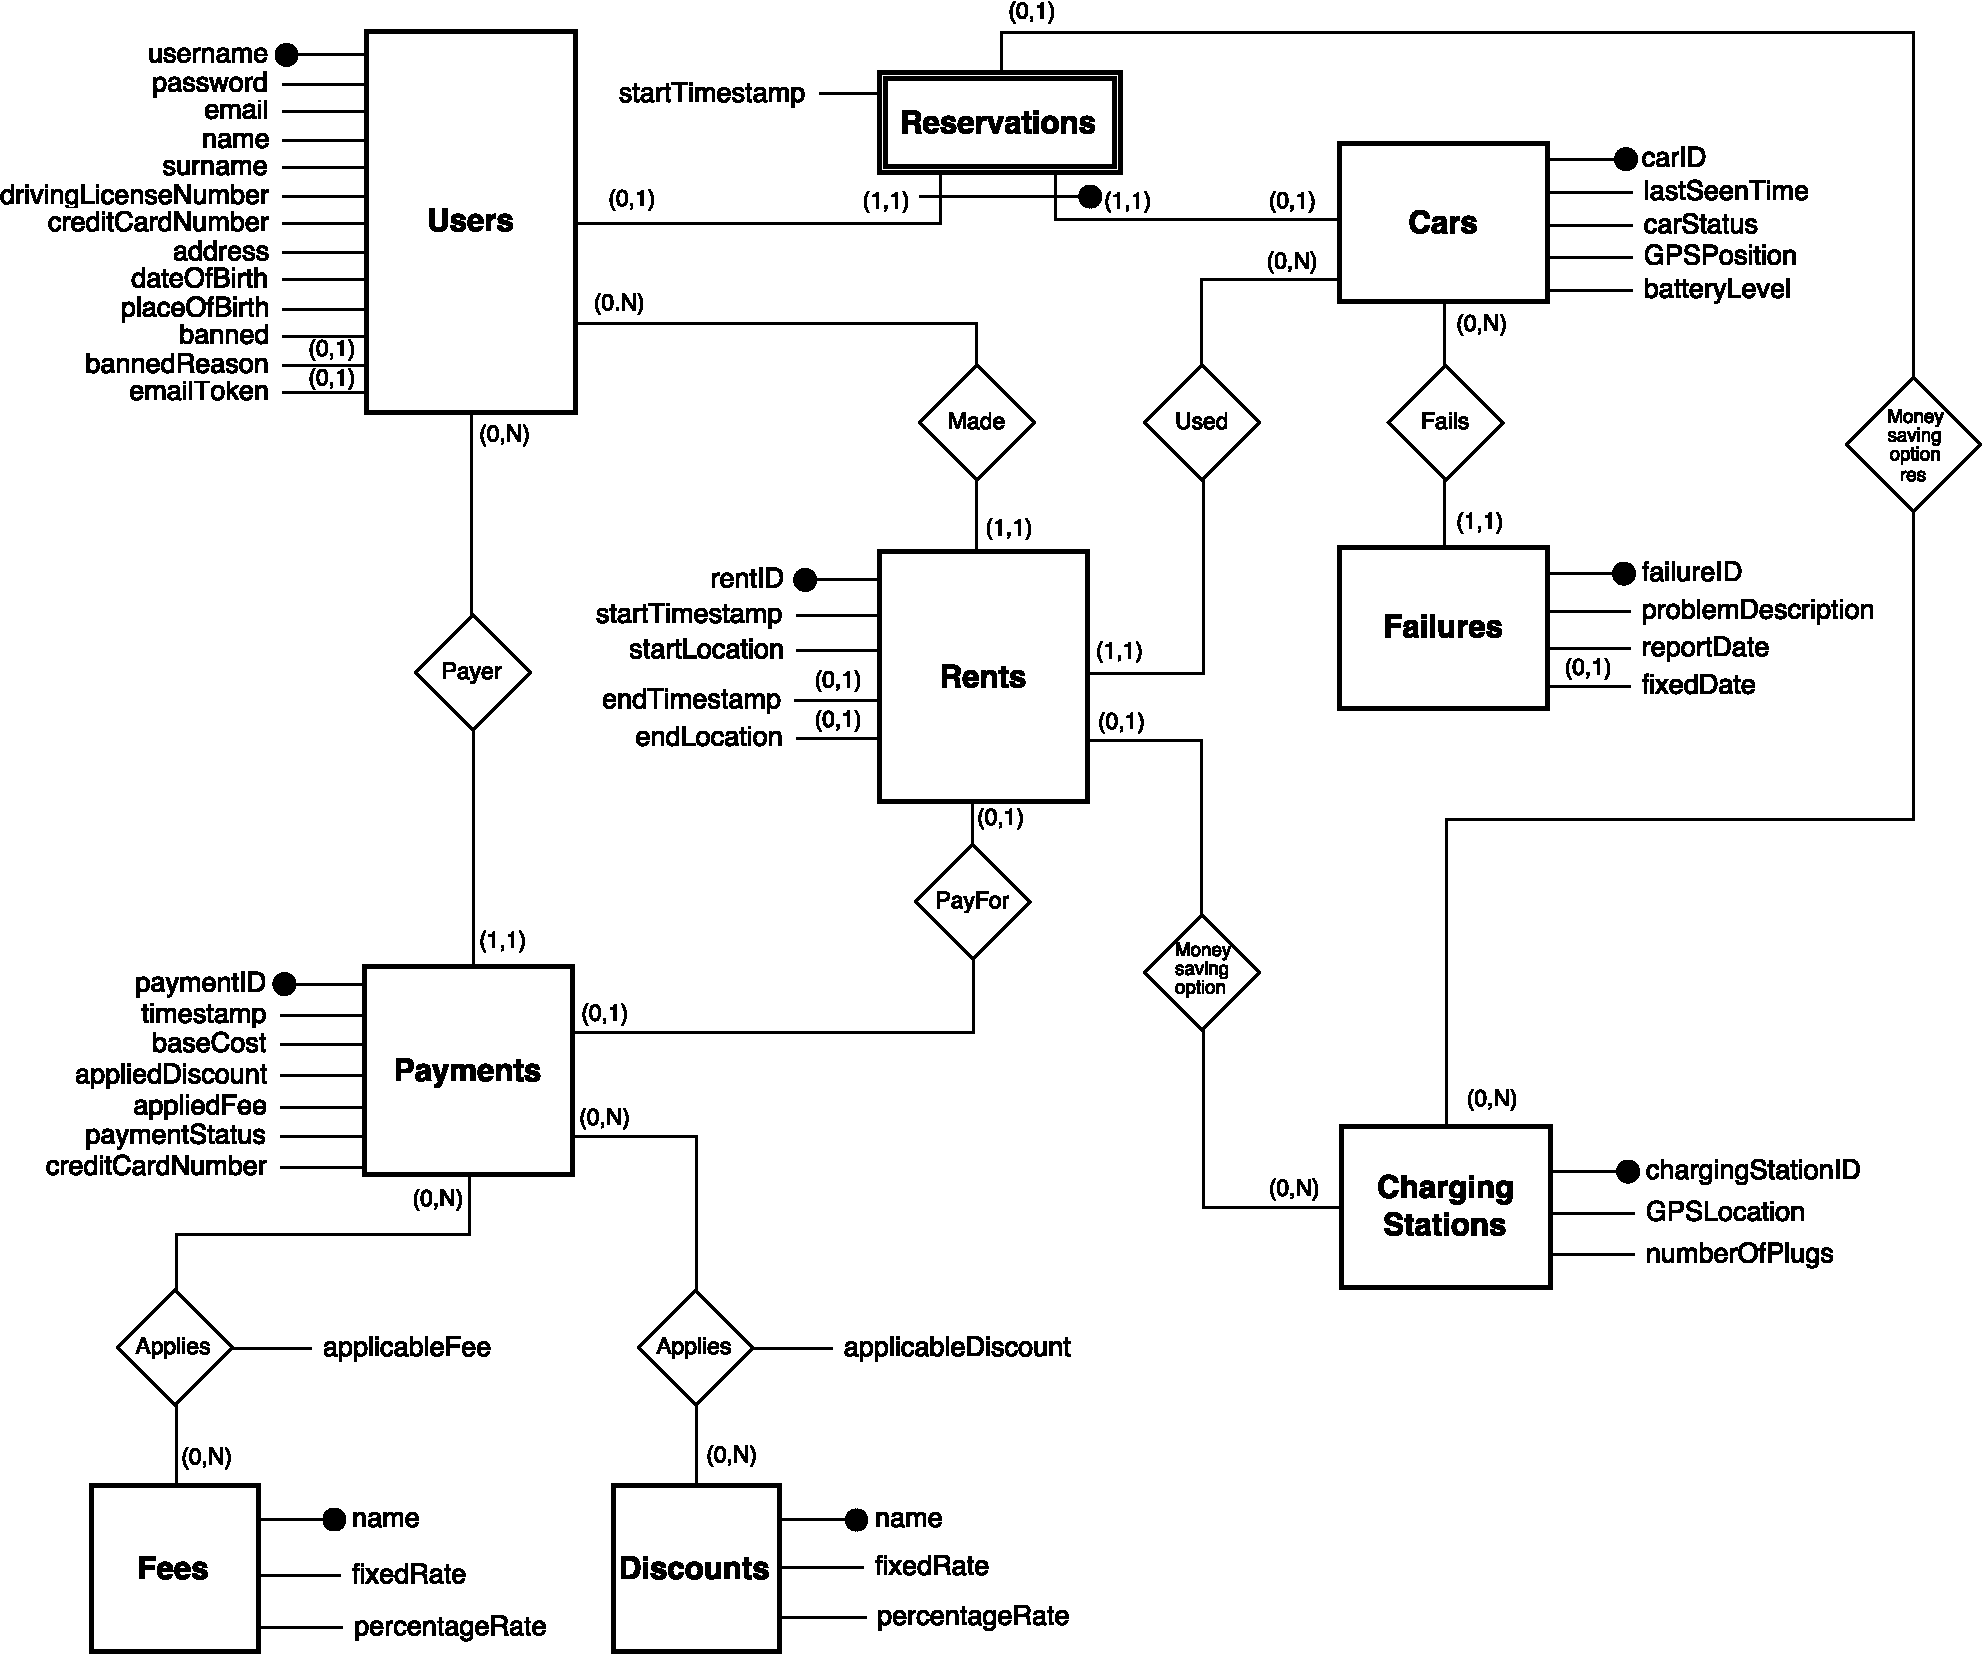
\includegraphics[width=0.9685\linewidth]{ER}
	\caption{
		\label{fig:ERModel} 
		ER model
	}
\end{figure}

\paragraph{Users} Beyond the primary key, the \mbox{\emph{email}}, \mbox{\emph{drivingLicenseNumber}} and \mbox{\emph{emailToken}} attributes must be unique.

\paragraph{Fees and discounts}
Fees and discounts must be defined as sum of a fixed value and a percentage factor w.r.t. the base rent cost.
The \emph{appliedDiscount} and \emph{appliedFee} payment attributes are determined, respectively, based upon the set of all \emph{applicableDiscount} and \emph{applicableFee} attributes associated to the rent. See \hyperref[sec:paymentAlgorithms]{payment algorithms} for more details.

As particular example, the \emph{OutOfSafeArea} fee, which is composed by a fixed amount plus a variable amount proportional to the \emph{distance} of the car form the nearest safe area, can be expressed as a fixed number of fees clustered w.r.t. distance.

\paragraph{Cars}Beyond the primary key, the \mbox{\emph{licenseNumber}} attribute must be unique. The \mbox{\emph{lastSeen}} attribute is set by default to the timestamp of the last car information update. The \mbox{\emph{carStatus}} attribute represents the car statuses as defined in the RASD.

\paragraph{Payment status} There are three possible payment status:
\begin{itemize}
	\item \emph{Pending}: a payment transaction request has been sent to the external payment system
	\item \emph{Confirmed}: the payment transaction has been successfully executed
	\item \emph{Rejected}: the payment transaction has failed
\end{itemize}
The default state for a payment is \emph{Pending}.

\paragraph{Failures}A failure is considered "open" (i.d. to be fixed) if the attribute \emph{fixedDate} is not present. A car can have at most one open failure.

\paragraph{Charging stations}Charging stations are provided to the system as an XML file with the following DTD:
\lstset{language=XML,frame=false}
\begin{lstlisting}
<!ELEMENT ChargingStations(ChargingStation+)>
<!ELEMENT ChargingStation(GPSLocation, NumberOfPlugs)>
<!ELEMENT GPSLocation(lat,long)>
<!ELEMENT lat(#CDATA)>
<!ELEMENT long(#CDATA)>
<!ELEMENT NumberOfPlugs(#CDATA)>
<!ATTLIST ChargingStation id ID #REQUIRED>
\end{lstlisting}
An example of such an XML file is 
\lstset{language=XML, frame=false, morekeywords={ChargingStations,ChargingStation,GPSLocation,NumberOfPlugs,lat,long}}
\begin{lstlisting}
<ChargingStations>

	<ChargingStation id="1">
		<GPSLocation>
			<lat>45.477452</lat>
			<long>9.218617</long>
		</GPSLocation>
		<NumberOfPlugs>10</NumberOfPlugs>
	</ChargingStation>
	
	<ChargingStation id="2">
		<GPSLocation>
			<lat>45.476257</lat>
			<long>9.171926</long>
		</GPSLocation>
		<NumberOfPlugs>15</NumberOfPlugs>
	</ChargingStation>
	
</ChargingStations>
\end{lstlisting}

\paragraph{Safe areas}Safe areas are also provided as XML file according to the \emph{GPX GPS Exchange Format} \cite{gpx} and they are composed by closed polygonal chains.

\paragraph{Safe areas and charging stations deployment}The position of charging stations and safe areas are processed and sent to cars only in case of:
\begin{itemize}
	\item system initialization (sent to all cars)
	\item changes in XML files (sent to all cars)
	\item new car (sent to one car)
\end{itemize}

\paragraph{Security}Users' passwords and all credit card numbers (associated to users and used for past payments) must be stored with proper and secure encryption.

\subsubsection{Server component}
To explain how the Server component manages interfaces, communication with external components and system functionalities we represent in \autoref{fig:ServerComponent} its internal structure showing its main components and their interactions.
\\

\begin{figure}[h]
			\centering
			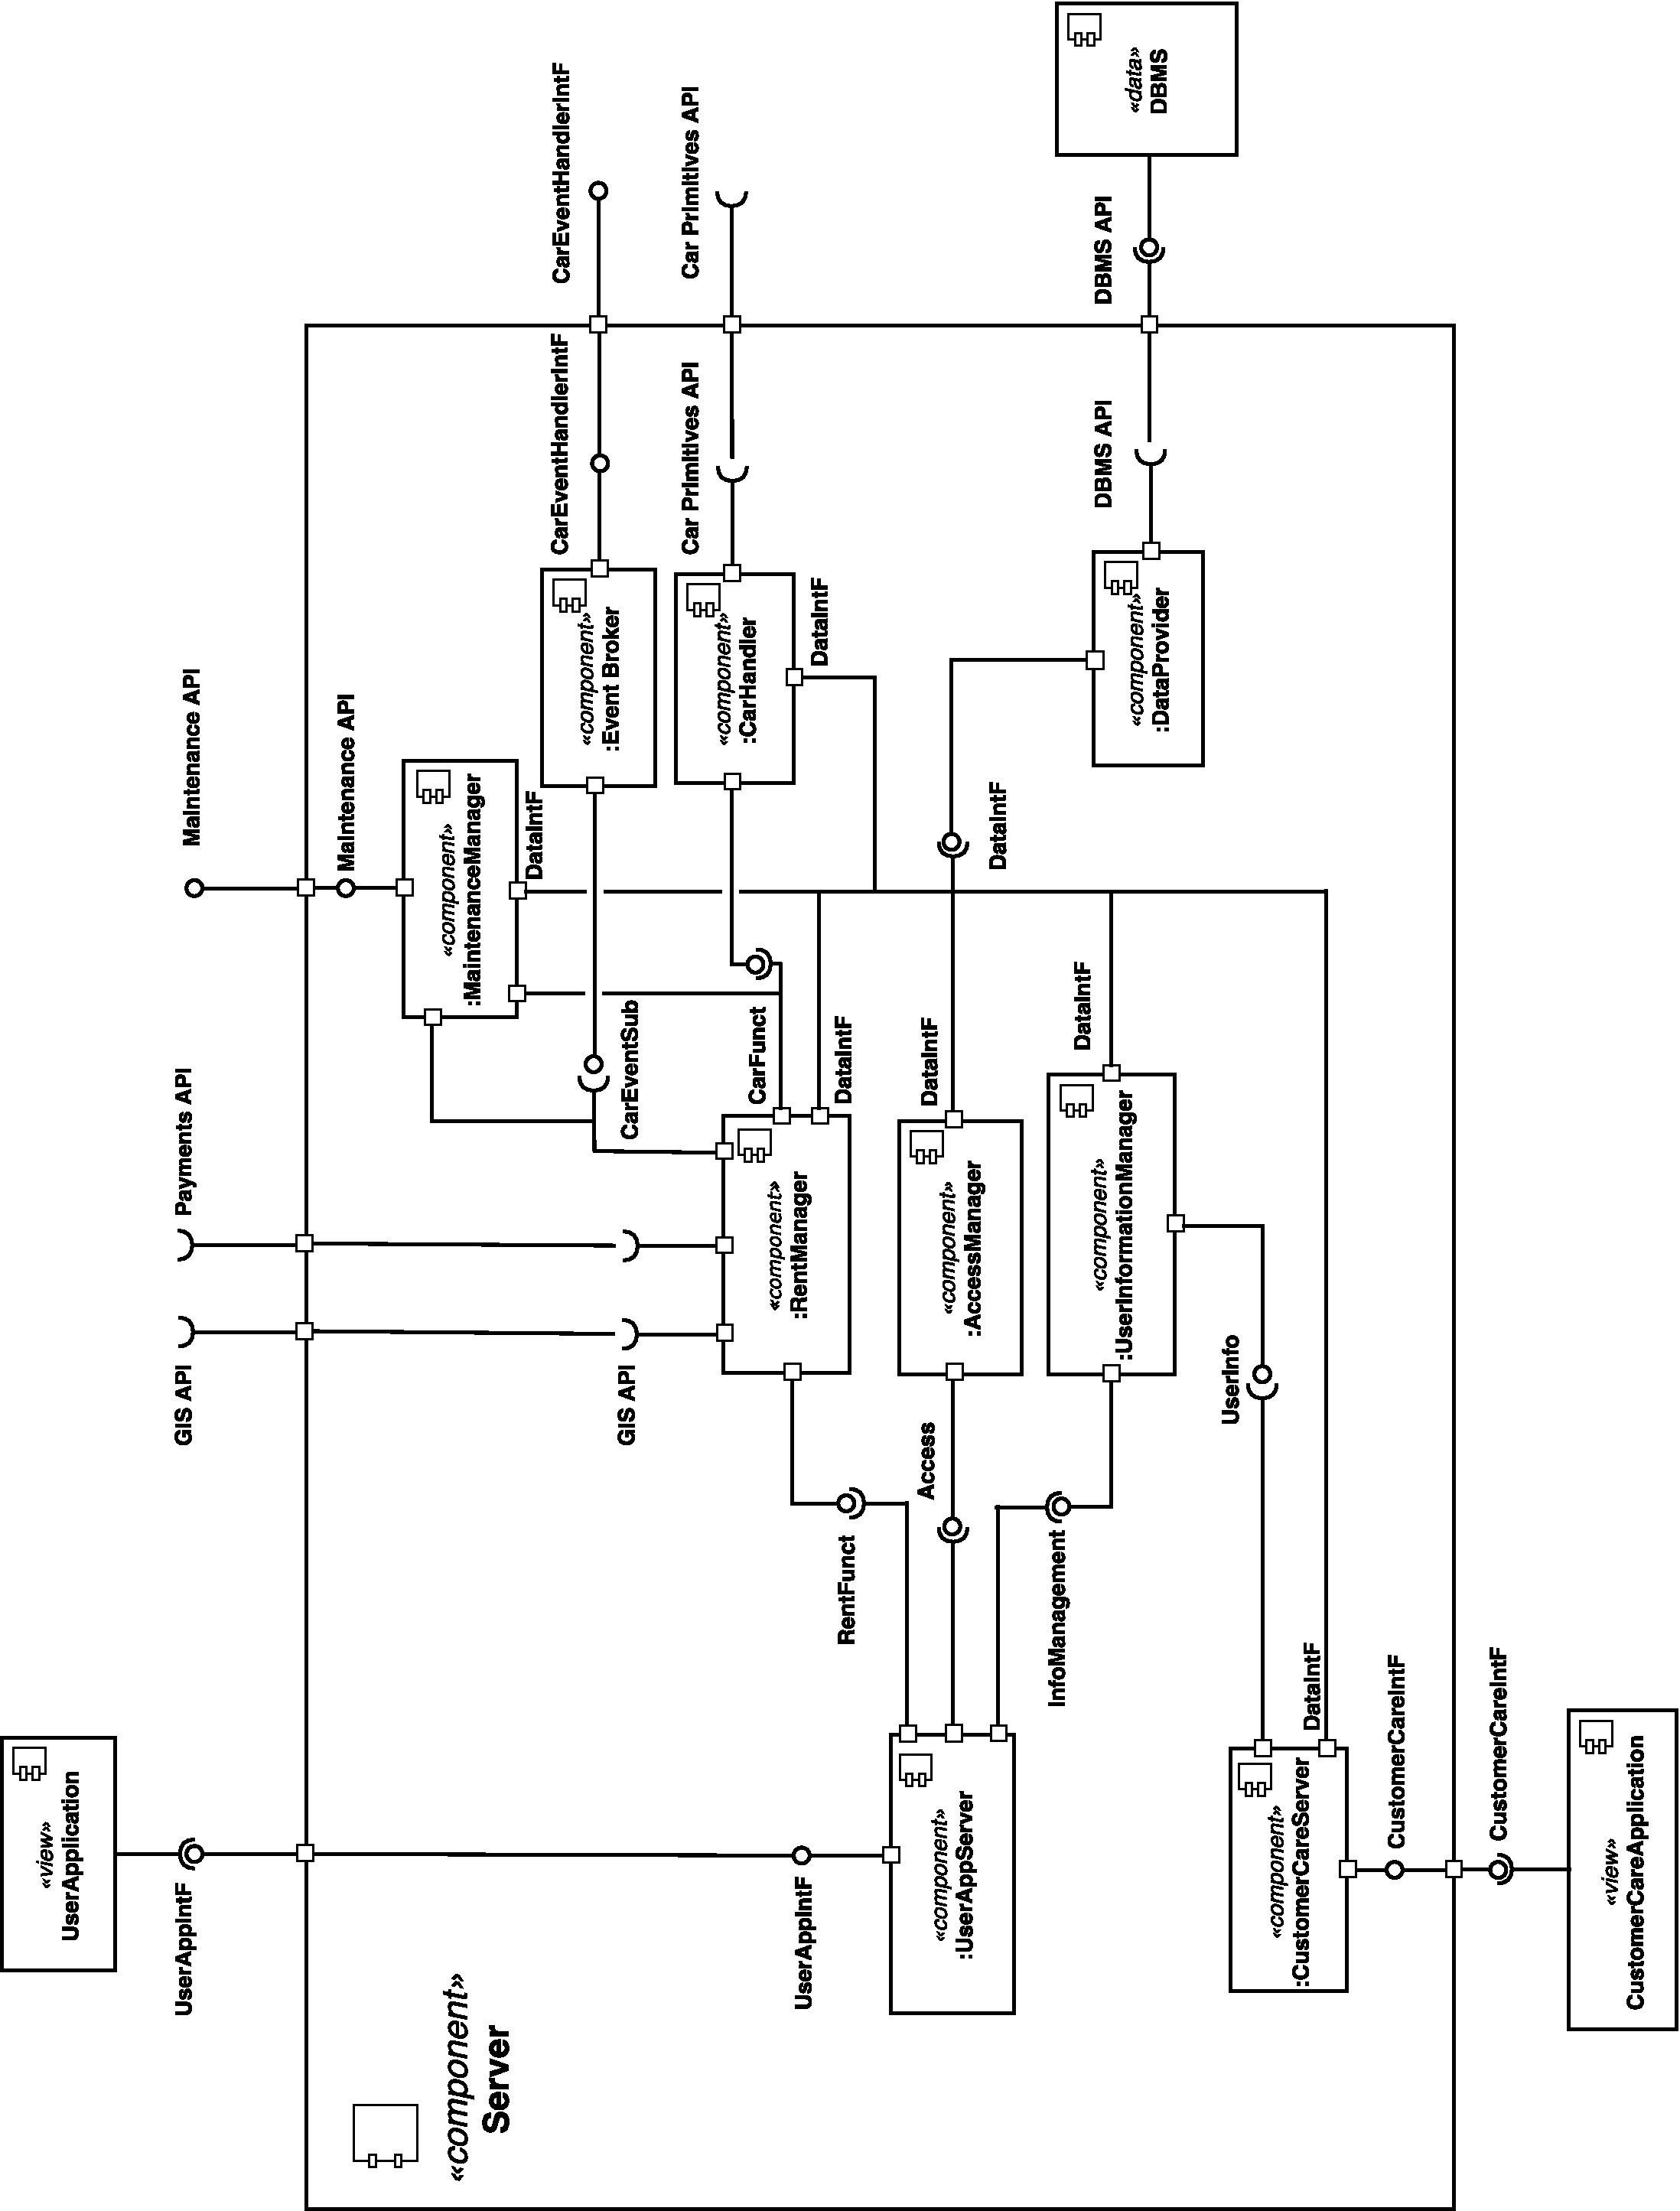
\includegraphics[angle=90,width=0.9685\linewidth]{ServerComponent}
			\caption{
				\label{fig:ServerComponent} 
				Server component
			}
		\end{figure}
\clearpage

This white box representation shows the parts composing the \emph{Server} component and their interactions by means of lollipop-socket notation. When designing this component's internal structure several concerns and requirements were taken into account:
\begin{itemize}
	\item all of its required and provided interfaces had to be delegated to some part of its internal structure
	\item all of the functionalities related to the car reservation, unlock, use and rent payment had to be addressed and provided by some parts of this component
	\item it had to communicate in different ways with different components, so interface specific parts had to be designed
	\item associations between internal components needed to be clarified, so lollipop-socket notation was used to express the provided or required interfaces of each part
\end{itemize}

\subsubsection{RentManager component}

\autoref{fig:rentObjectDiagram} shows the internal structure of the Rent Manager component; an \mbox{Object} \mbox{Diagram} was used in order to show the objects realizing the component functionalities and the associations between the aforementioned objects. This diagram also shows the delegation associations between the provided and required interfaces of the components and the objects realizing it.
\\
This component encapsulates most of the logic of the System, it manages the information coming from the cars and it creates and manages rents and payments. 

\begin{figure}[h!]
	\centering
	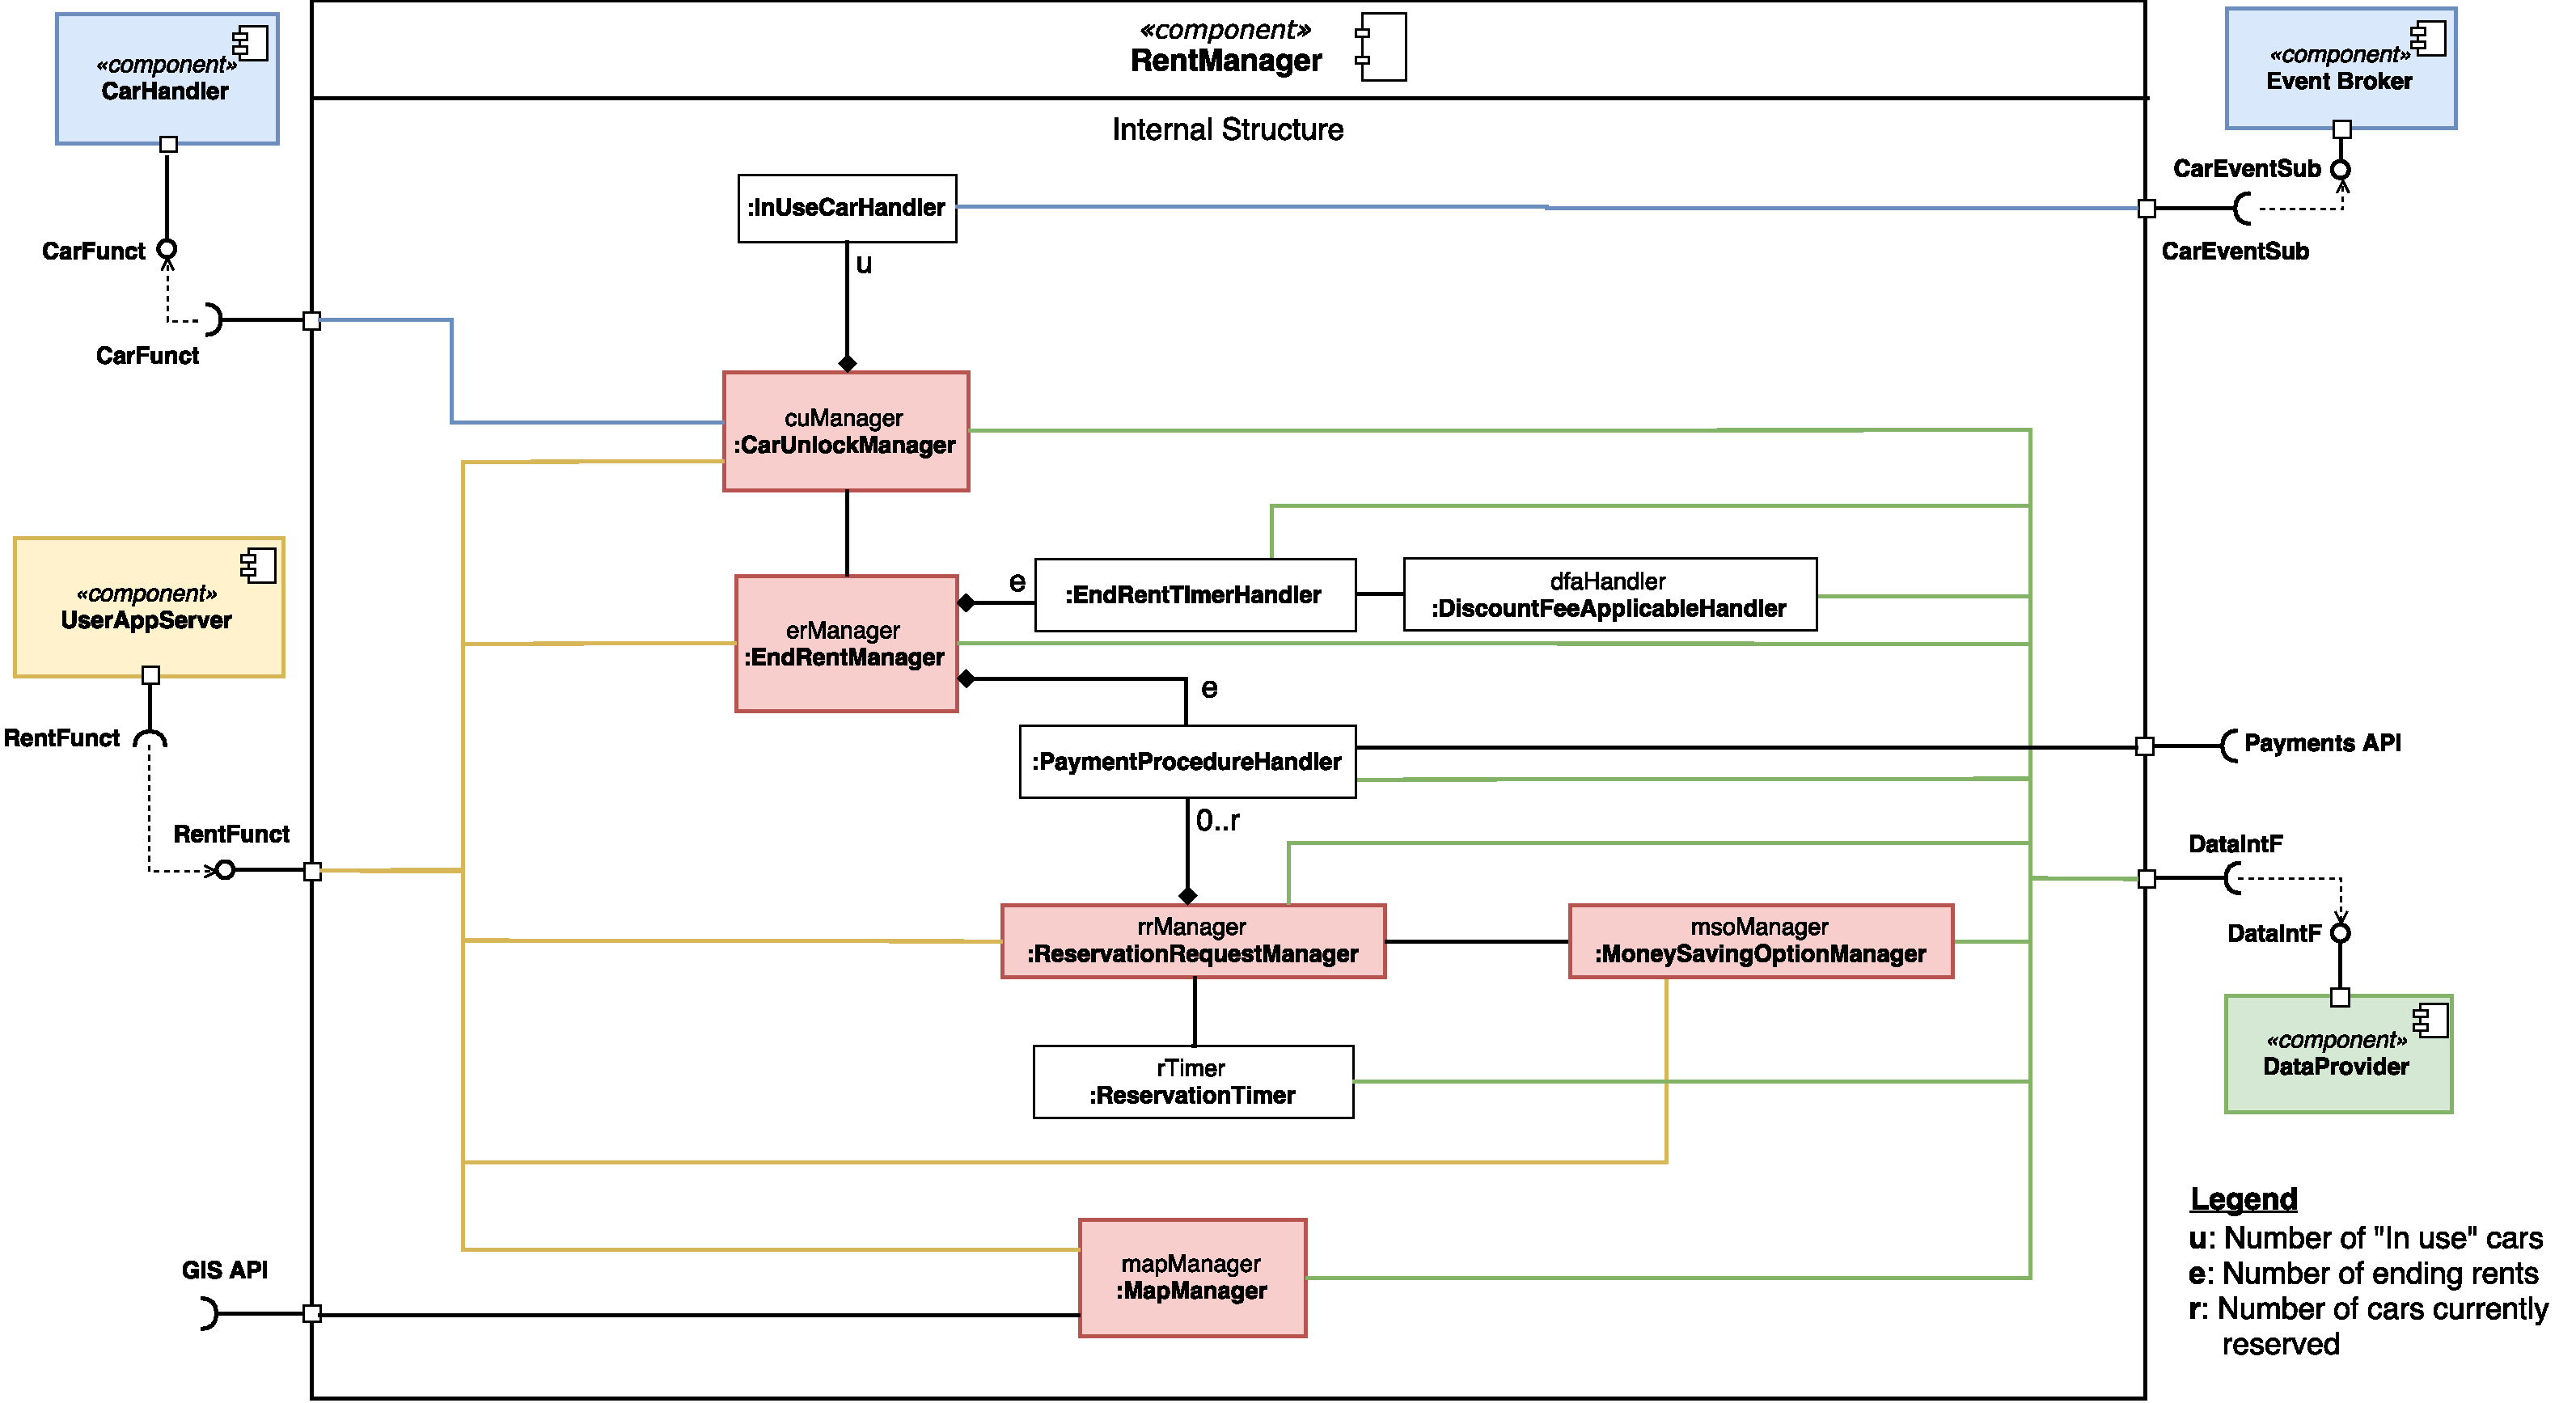
\includegraphics[angle=90,width=0.7\linewidth]{ObjectRentManager}
	\caption{
		\label{fig:rentObjectDiagram} 
		\emph{RentManager} object diagram
	}
\end{figure}

\paragraph{InUseCarHandler:} this part of the RentManager manages in use cars, it subscribes to the events of a specific car through the EventBroker component which enables asynchronous communication between the cars and the system.
\paragraph{CarUnlockManager:} this part of the RentManager is the one that manages the unlock car requests, it checks, by accessing the DataProvider component, that the user who is requesting the unlock actually reserved the car and that he is less than 5 meters away from it; after that it activates the necessary triggers on the car and instantiate an InUseCarHandler object which will subscribe to them. When a rent ends the CarUnlockManager is notified by the corresponding InUseCarHandler, it will update the status of the car and it will notify the EndRentManager component in order to terminate the rent.
\paragraph{EndRentManager:} this part of the RentManager is the one that manages the termination of the rent and that starts the payment procedure via the \mbox{PaymentProcedureHandler} object.
\paragraph{ReservationRequestManager:} this part of the RentManager component is the one in charge of receiving and validating the reservation requests made by users.
\paragraph{PaymentProcedureHandler:} this part of the RentManager allows other components to instantiate payments and interacts with the External Payment System in order to realize them.
\paragraph{ReservationTimer:} this part of the RentManager component checks if any reservation expires and if so it instantiate a ProcedureHandeler in order to make the user pay the fee for the expiration.
\paragraph{MoneySavingOptionHandler:} this component is used by the ReservationRequestManager when a user enables the Money Saving Option in his reservation; given the user's destination it calculates the most convenient Charging Station and it returns it to the ReservationRequestManager.
\paragraph{EndRentTimerHandler:} this timer is used to let the user connect the car to a power plug after his rent has ended; if a car is connected to the power plug after this timer has expired, the user won't receive the related discount.
\paragraph{DiscountFeeApplicableHandler:} this part of the RentManager component is used by the EndRentTimerHandler at the end of the rent and it checks which Discounts and which Fees are applicable to the rent.

\clearpage
\subsubsection{MaintenanceManager component}
\autoref{fig:maintenanceManagerObjectDiagram} shows the internal structure of the Maintenance Manager component; an Object Diagram was used in order to show the objects realizing the component functionalities and the associations between the aforementioned objects. This diagram also shows the delegation associations between the provided and required interfaces of the components and the objects realizing it.
\\
This component provides the Maintenance Service with all the functionalities it needs, granting it access to the API and allowing it to see unavailable cars and tag fixed cars as available.
\begin{figure}[h!]
	\centering
	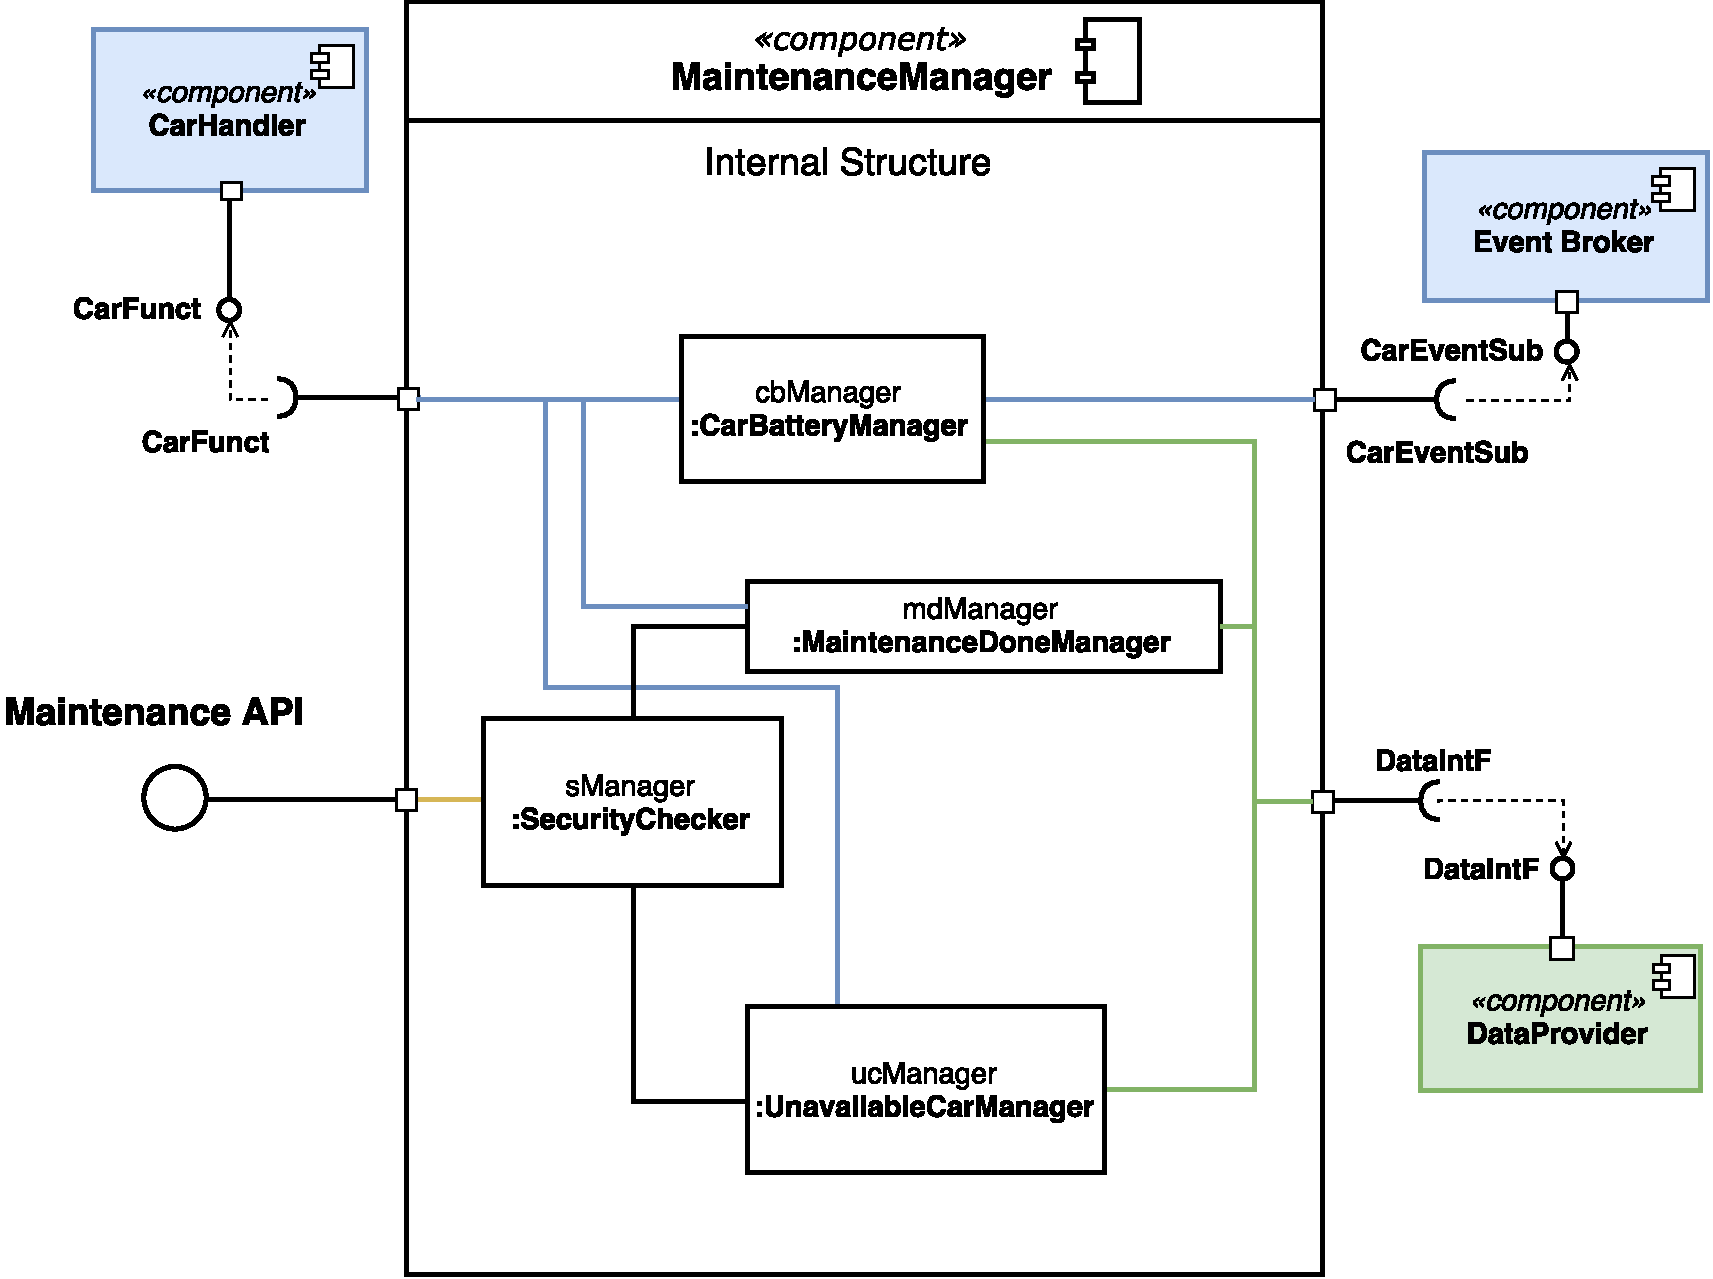
\includegraphics[width=\linewidth]{ObjectMaintenanceManager}
	\caption{
		\label{fig:maintenanceManagerObjectDiagram} 
		\emph{MaintenanceManager} object diagram
	}
\end{figure}

\paragraph{CarBatteryManager:} this part of the MaintenanceManager component can check the battery status of the cars and be notified by them when their battery level is critical.
\paragraph{SecurityChecker:} this part of the MaintenanceManager componenent is in charge of ensuring that only the Maintenance Service is able to access the services offered by the API.
\paragraph{UnavailableCarManager:} this part of the MaintenanceManager component builds the list of \emph{Not available} cars from the database and for each car of the list generates software keys to let maintenance operators to access those cars.
\paragraph{MaintenanceDoneManager:} this part of the MaintenanceManager component allows the Maintenance Service operators to tag a car as \emph{Available} after fixing a problem.

\subsubsection{UserInformationManager component}
\autoref{fig:userInformationManagerObjectDiagram} shows the internal structure of the UserInformationManager component; an Object Diagram was used in order to show the objects realizing the component functionalities and the associations between the aforementioned objects. This diagram also shows the delegation associations between the provided and required interfaces of the components and the objects realizing it.
This component manages the user information present in the system, granting access to it to the Customer Care and to the User Application Server.
\begin{figure}[h!]
	\centering
	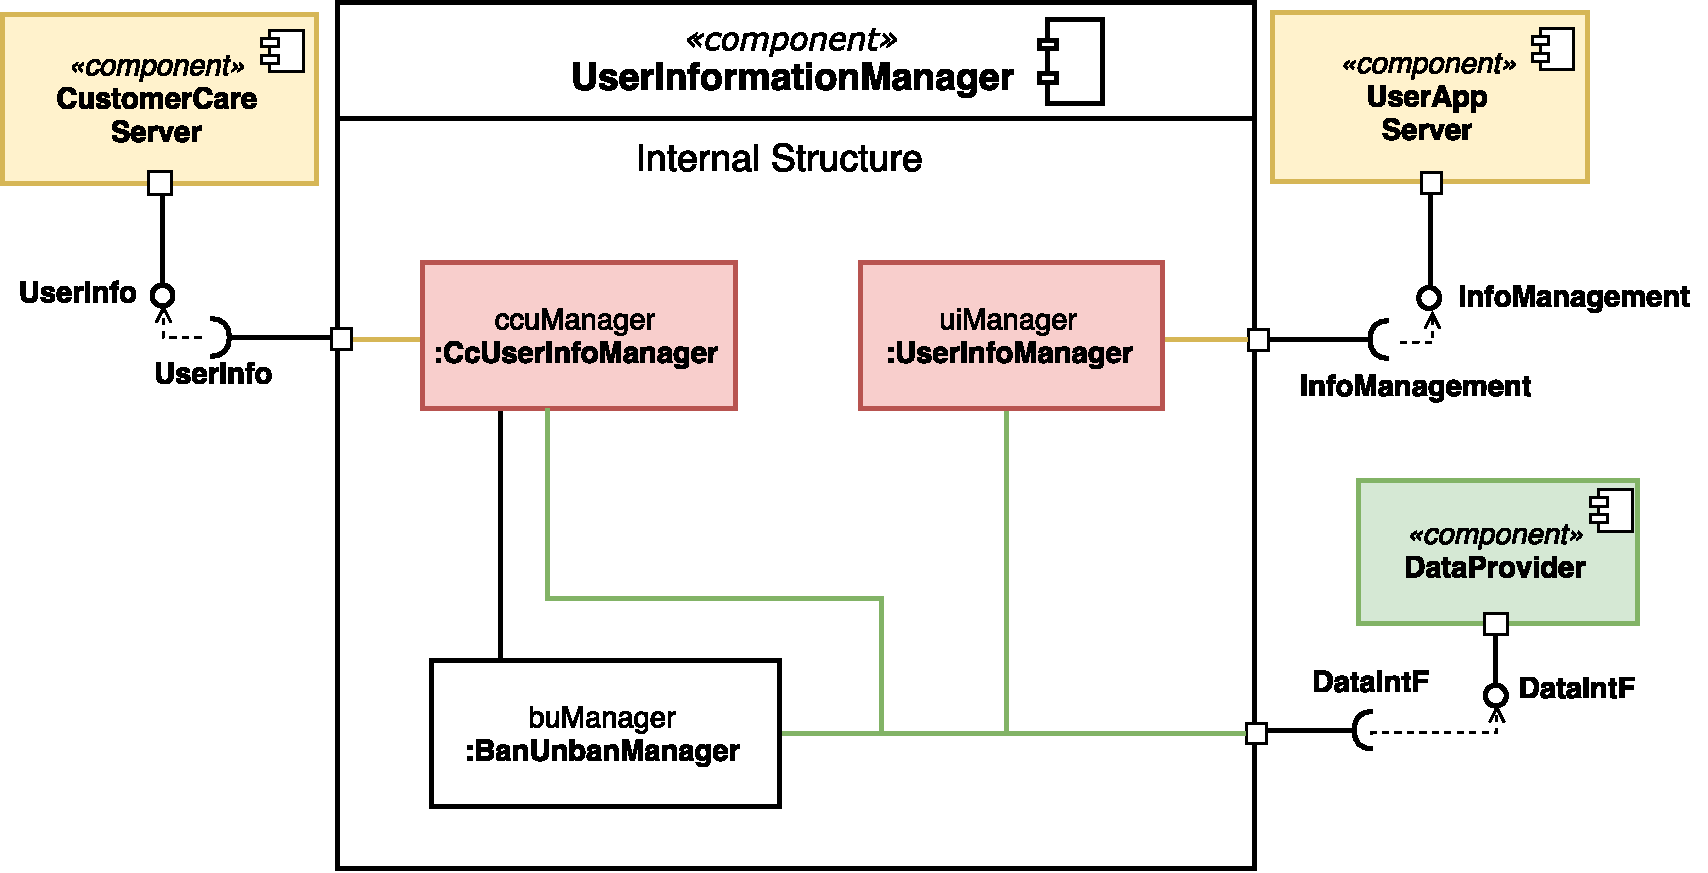
\includegraphics[width=\linewidth]{ObjectUserInformationManager}
	\caption{
		\label{fig:userInformationManagerObjectDiagram} 
		\emph{UserInformationManager} object diagram
	}
\end{figure}

\paragraph{CcUserInfoManager:} this part of the UserInformationManager component provides the Customer Care with the information it is allowed to access, and allows it access the BanUnbanManager.
\paragraph{UserInfoManager:} this part of the UserInformationManafer component provides the User Application Server with the information it is allowed to access.
\paragraph{BanUnbanManager:} allows the Customer Care to ban or unban Users.
\subsubsection{AccessManager component}
This component manages the registration and login phase of users, it encapsulates the logic that allows the users to register and login. Having a component for this specific purpose enhances decoupling in the system and ensures that these functionalities will not be affected by changes in other components of the system.

\subsubsection{UserAppServer component}
This component acts as an interface between the user and the application logic of the system; it produces the html pages shown to the user by his web browser and it receives the commands the users inputs on the web page. This component solves the concerns related to the handling of the requests sent by the users: these connection requests and the work related to generating the web pages will be handled by this component, without causing load problems on the application logic. It also allows the decoupling of the application logic from the presentation logic, which has to be realized in a four tier client-server architecture.

\subsubsection{CustomerCareServer component}
This component provides the CustomerCareApplication client with the information it needs to show and with the functionalities it needs to access; this component was decoupled from the UserAppServer component because it offers different functionalities and is only used and accessible by a specific client application.

\subsubsection{DataProvider component}
This component is in charge of providing a unified interface to the different data sources of the System, both the DBMS and the files contained in the File System of the OS hosting the application logic. This component allows a better decoupling between the application logic components and the underlying data layer.

\subsubsection{CarHandler and EventBroker components}
These 2 components are responsible for the communication with the cars embedded system.
\paragraph{Car Handler} exposes to the PowerEnJoy system all of the primitives provided by the car embedded system; it does that via a client server communication in which the cars embedded system is the server, offering its primitives, and the CarHandler component is the client, requesting the primitives.
\paragraph{EventBroker} instead is notified by the cars embedded system when some specific events take place in the car system; this communication is realized via a publish subscribe paradigm in which the cars embedded system is the publisher, publishing events on the EventBroker component, and the internal components of the PowerEnJoy system are the subscribers which are interested to the events taking place in the cars. 
\clearpage

\subsection{Deployment view}

\subsubsection{Four tier architecture}
Taking into account that:
\begin{itemize}
	\item the \emph{Composition viewpoint} diagram shows the need of database decoupling from the actual system
	\item in the \emph{Server component view} we can clearly distinguish modules who take care of presentation and communication with the client
	\item in the \emph{Server component view} we can clearly distinguish modules who take care of the specific application logic
\end{itemize}
we decided to design the system on a four tier architecture pattern (see also \label{sec:deploymentView}
\begin{figure}[h!]
	\centering
	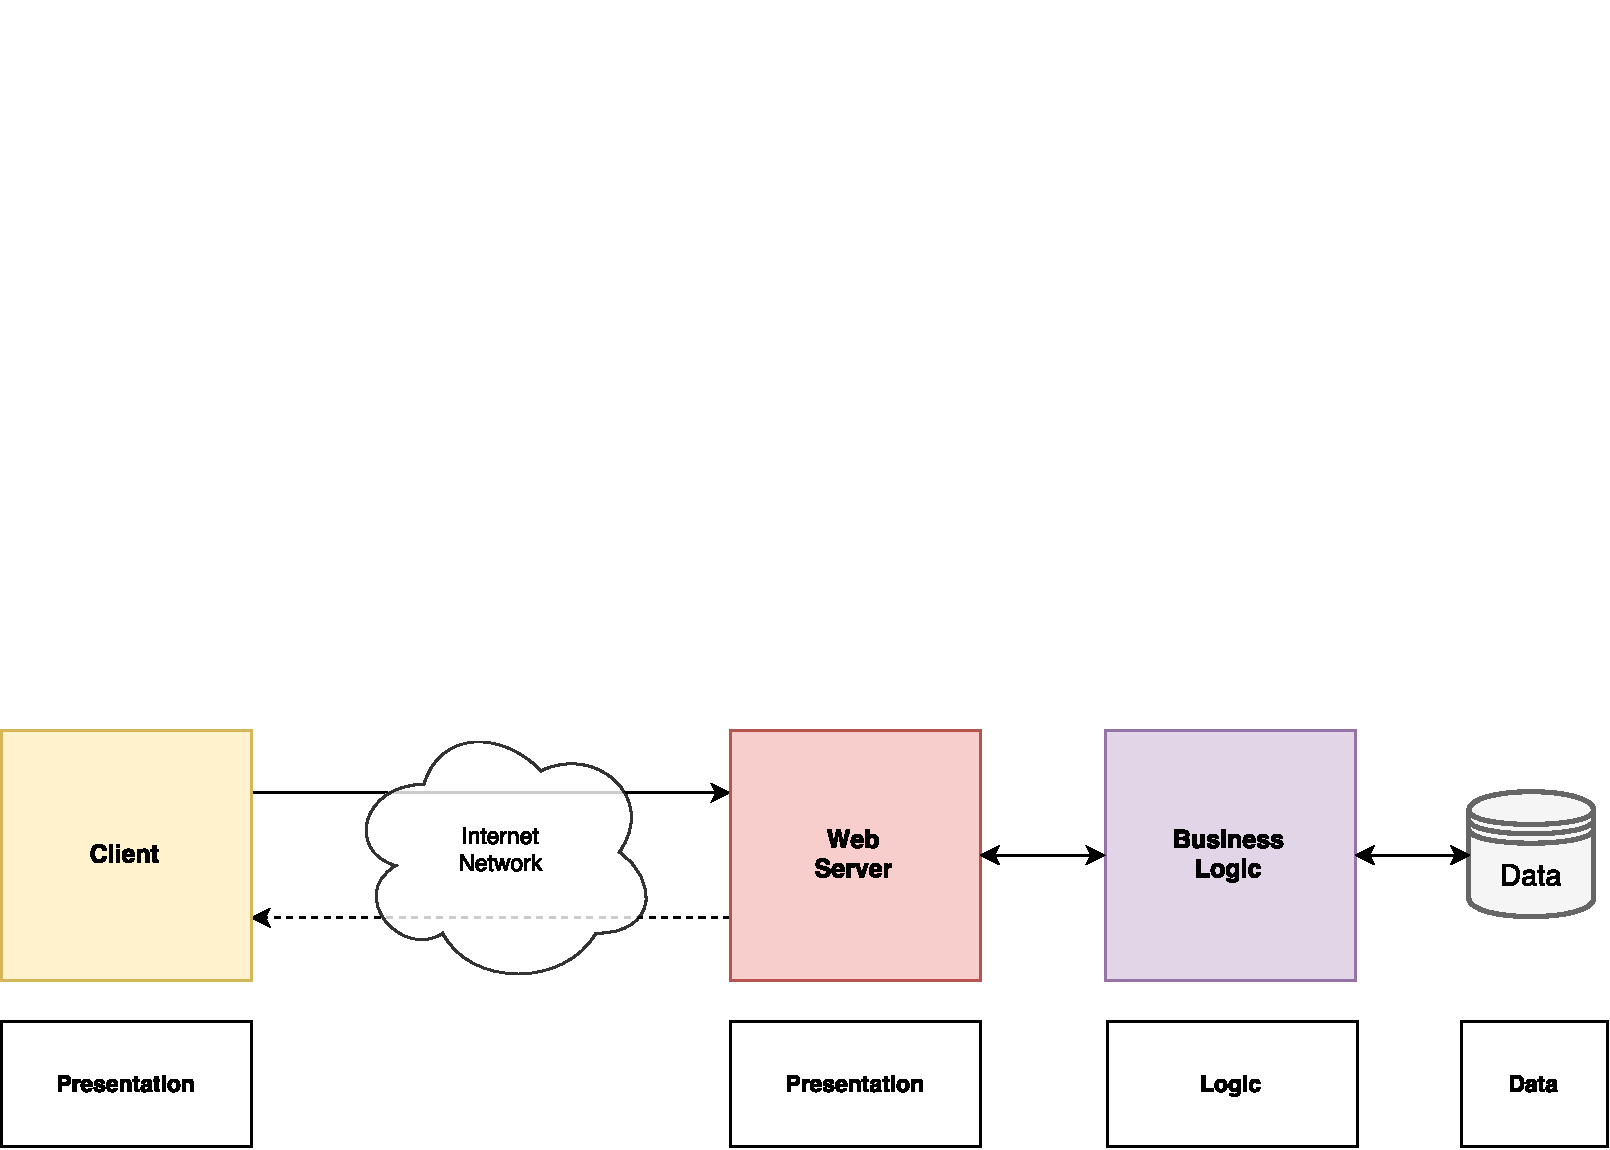
\includegraphics[width=\linewidth]{4Tier}
	\caption{
		\label{fig:fourTierCloud} 
		Four tier architecture with internet layer
	}
\end{figure}
\paragraph{Mapping of Server components on architecture:}to clarify at a finer level how the Server components are mapped in the four tier layered architecture the following diagram represents the Server components highlighted in the same color of the tier in the previous diagram:
\begin{itemize}
	\item Client: components used by users in order to access the functionalities offered by the system
		\begin{itemize}
			\item UserApplication
			\item CustomerCareApplication
		\end{itemize}
	\item Web Server: components which provides interfaces to clients in order to allow them to use functionalities offered by the system
		\begin{itemize}
			\item UserAppServer
			\item CustomerCareServer
		\end{itemize}
	\item Business Logic: components which realizes the functionalities offered by the system
		\begin{itemize}
			\item RentManager
			\item AccessManager
			\item UserInformationManager
			\item MaintenanceManager
			\item EventBroker
			\item CarHandler
			\item DataProvider
		\end{itemize}
	\item Data: components which store and manage the access to the data produced and needed by the Business Logic
		\begin{itemize}
			\item DBMS
		\end{itemize}
\end{itemize}

\begin{figure}[h]
			\centering
			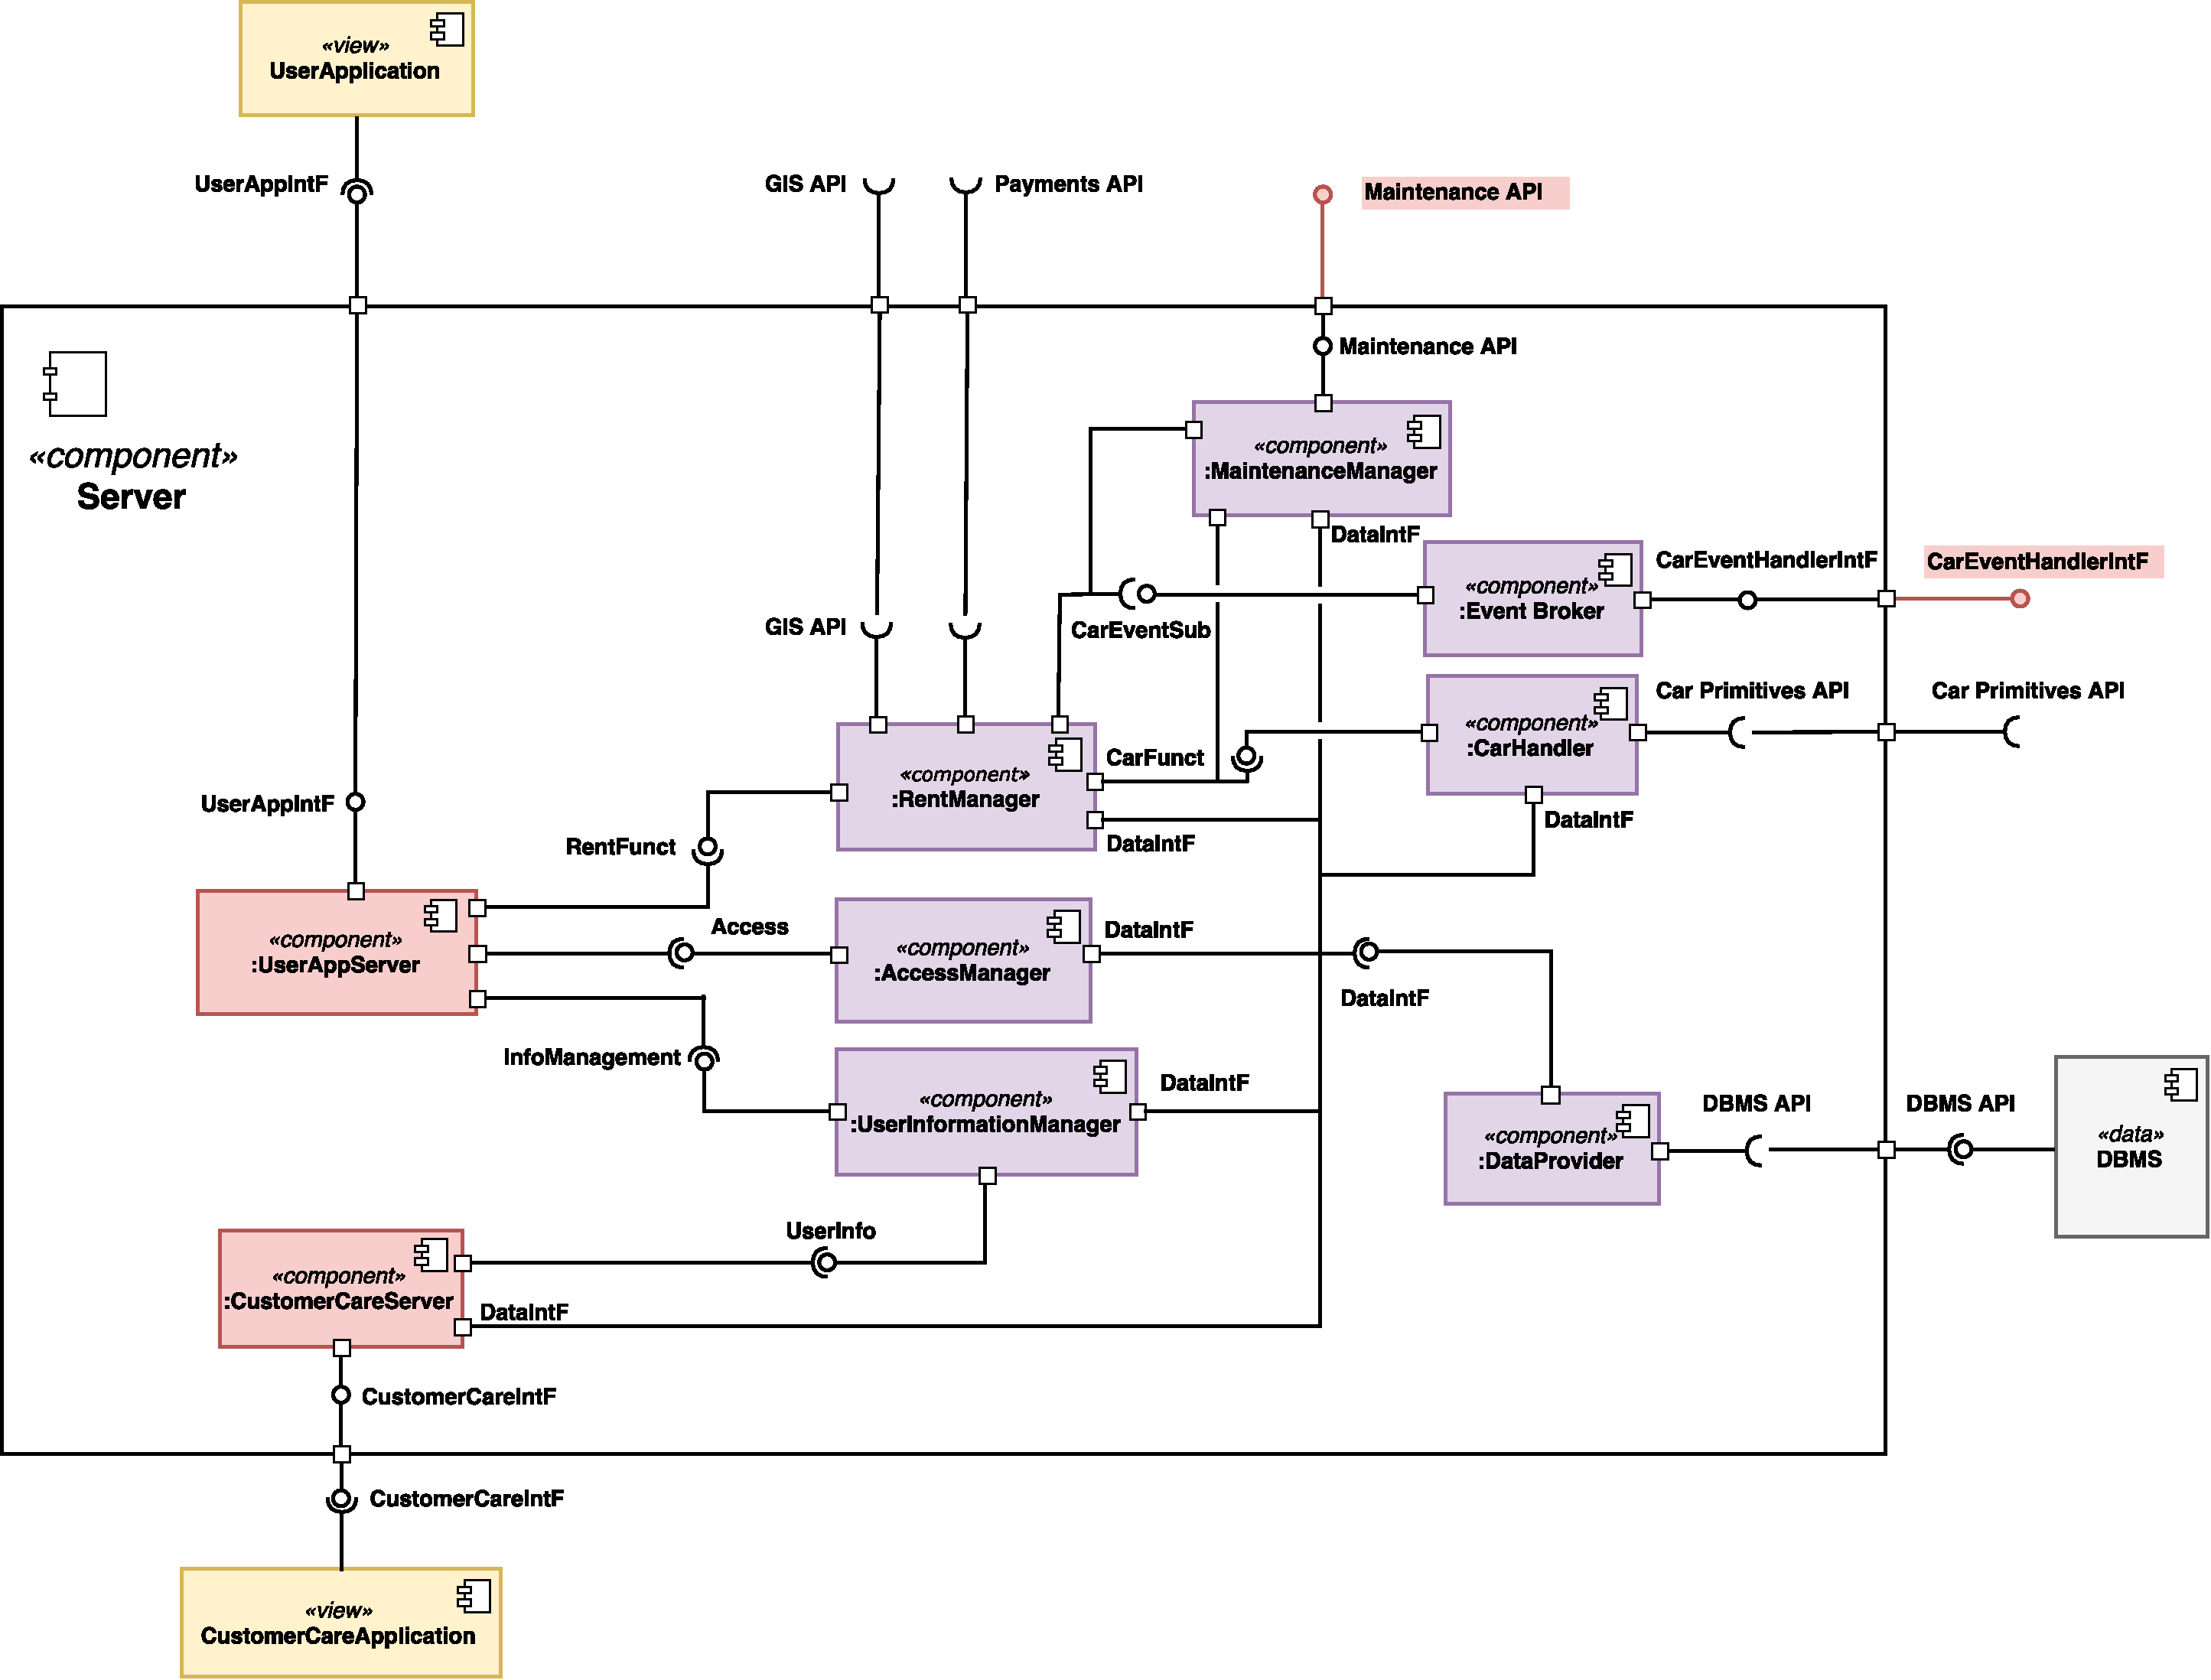
\includegraphics[angle=90,width=0.9685\linewidth]{deployComponent}
			\caption{
				\label{fig:deployServerComponent} 
				Mapping server component on architecture
			}
		\end{figure}
\clearpage

\subsubsection{Deployment diagram}
This diagram represents the mapping of the software components depicted in \autoref{fig:deployServerComponent} and \autoref{fig:highLevelComponents} on the devices that will run them. Many design concerns were considered while developing this solution.
\paragraph{Security:}security is ensured in different points of the architecture, in particular the UserAppServer uses HTTPS as communication protocol to communicate with the users; the devices running the CustomerCareApplication component are in a VPN with the device running the CustomerCareServer.
\paragraph{Scalability:}this model of deployment is scalable in the sense that the system administrators will be able to add more devices and deploy more instances of the needed components when and where performance issues will arise, in order to maintain a minimum level of performance even with loads increase.
\paragraph{Decoupling:}decoupling in this architecture is present at different levels; in the deployment diagram it is clear that the each of the four tier runs on different devices, moreover the UserAppServer component runs on a different device than the CustomerCareServer, the Maintenance API and the CarEventHandlerIntF.
\paragraph{Redundancy:}in this iteration of the architecture no redundancy of components or devices is present, but it is allowed in prevision of future expansions of the system's infrastructure.
\paragraph{Fault Tolerance:}deploying different components on different machines allows the system to be easier to recover in case of a problem on one of the machines; for an example the WebServer running the UserAppServer component goes down, it can be replaced with another machine and in the mean time the ApplicationServer would still be up and running and still be able to provide the CustomerCareApplication with its functionalities.

\begin{figure}[h!]
	\centering
	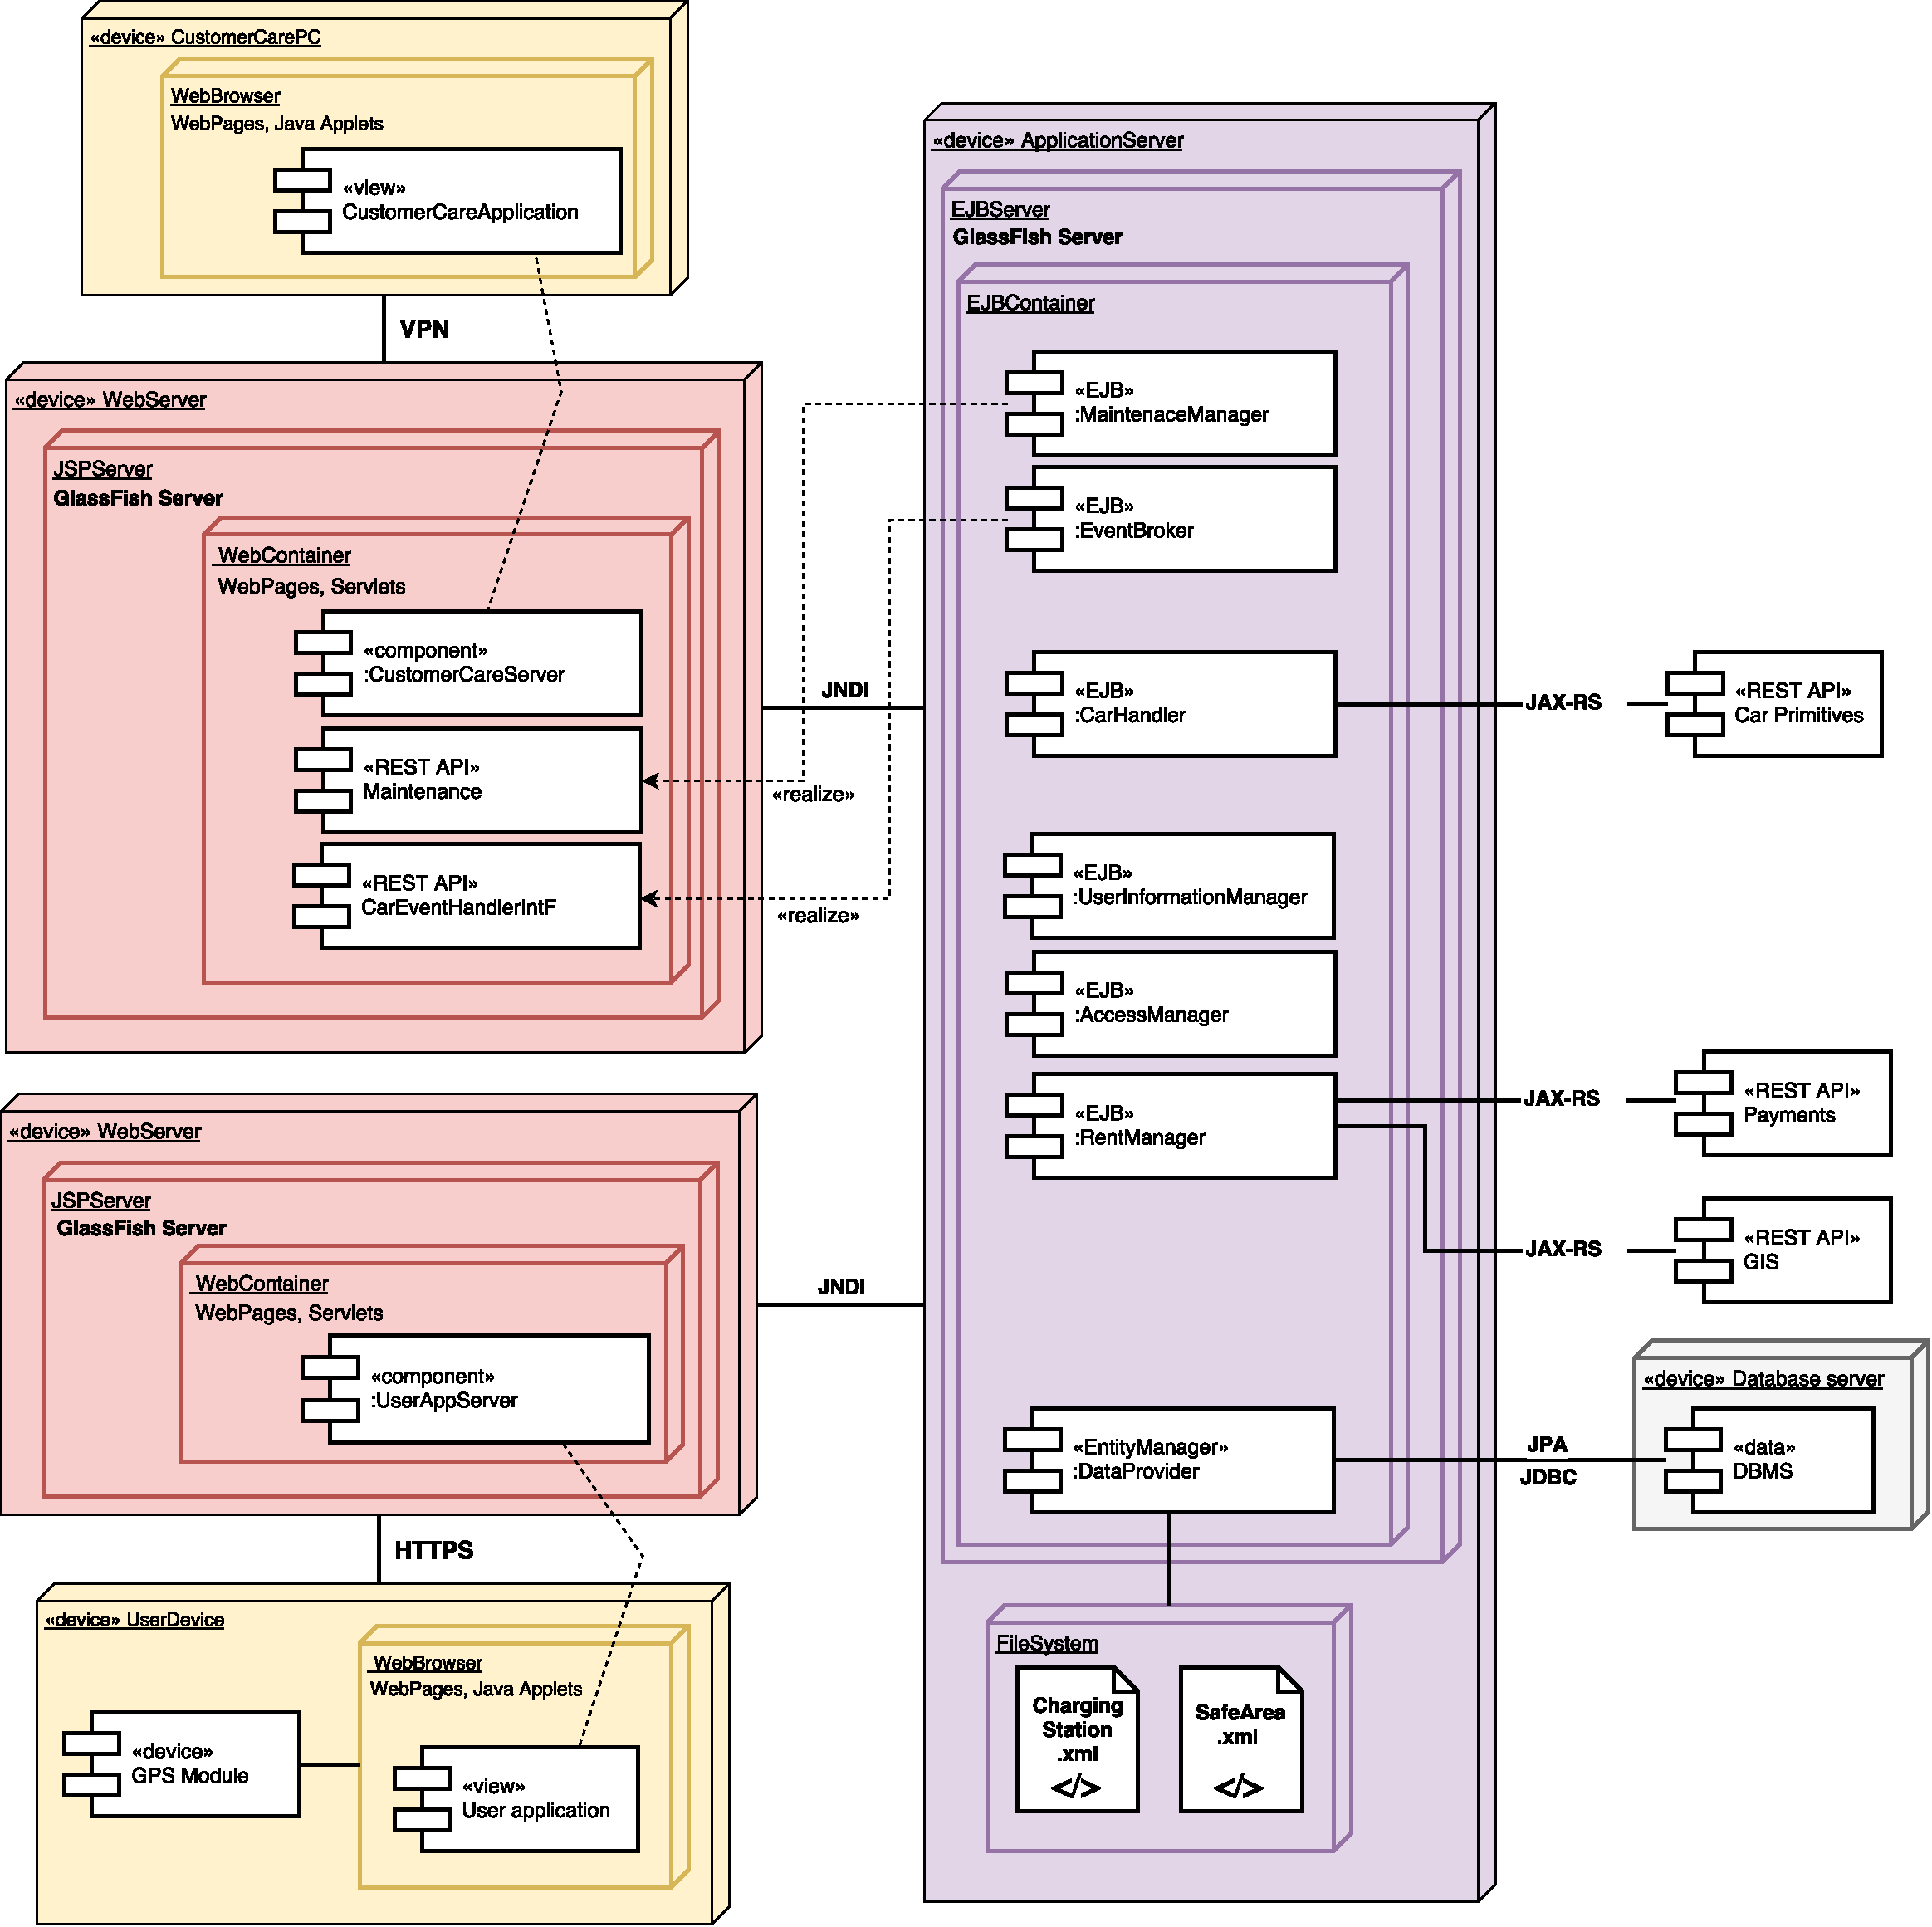
\includegraphics[width=\linewidth]{deployment}
	\caption{
		\label{fig:deployment} 
		Deployment diagram
	}
\end{figure}

\clearpage
\subsection{Runtime view}

\subsubsection{Map}
The \autoref{fig:mapGeneration} shows how the map is combined with safe areas, charging stations and available cars nearby a location given by the user.

The \emph{MapManager} component takes care of updating the battery level information of the car shown on the map which the system has not interacted with for the last two hours.

\begin{figure}[h!]
	\centering
	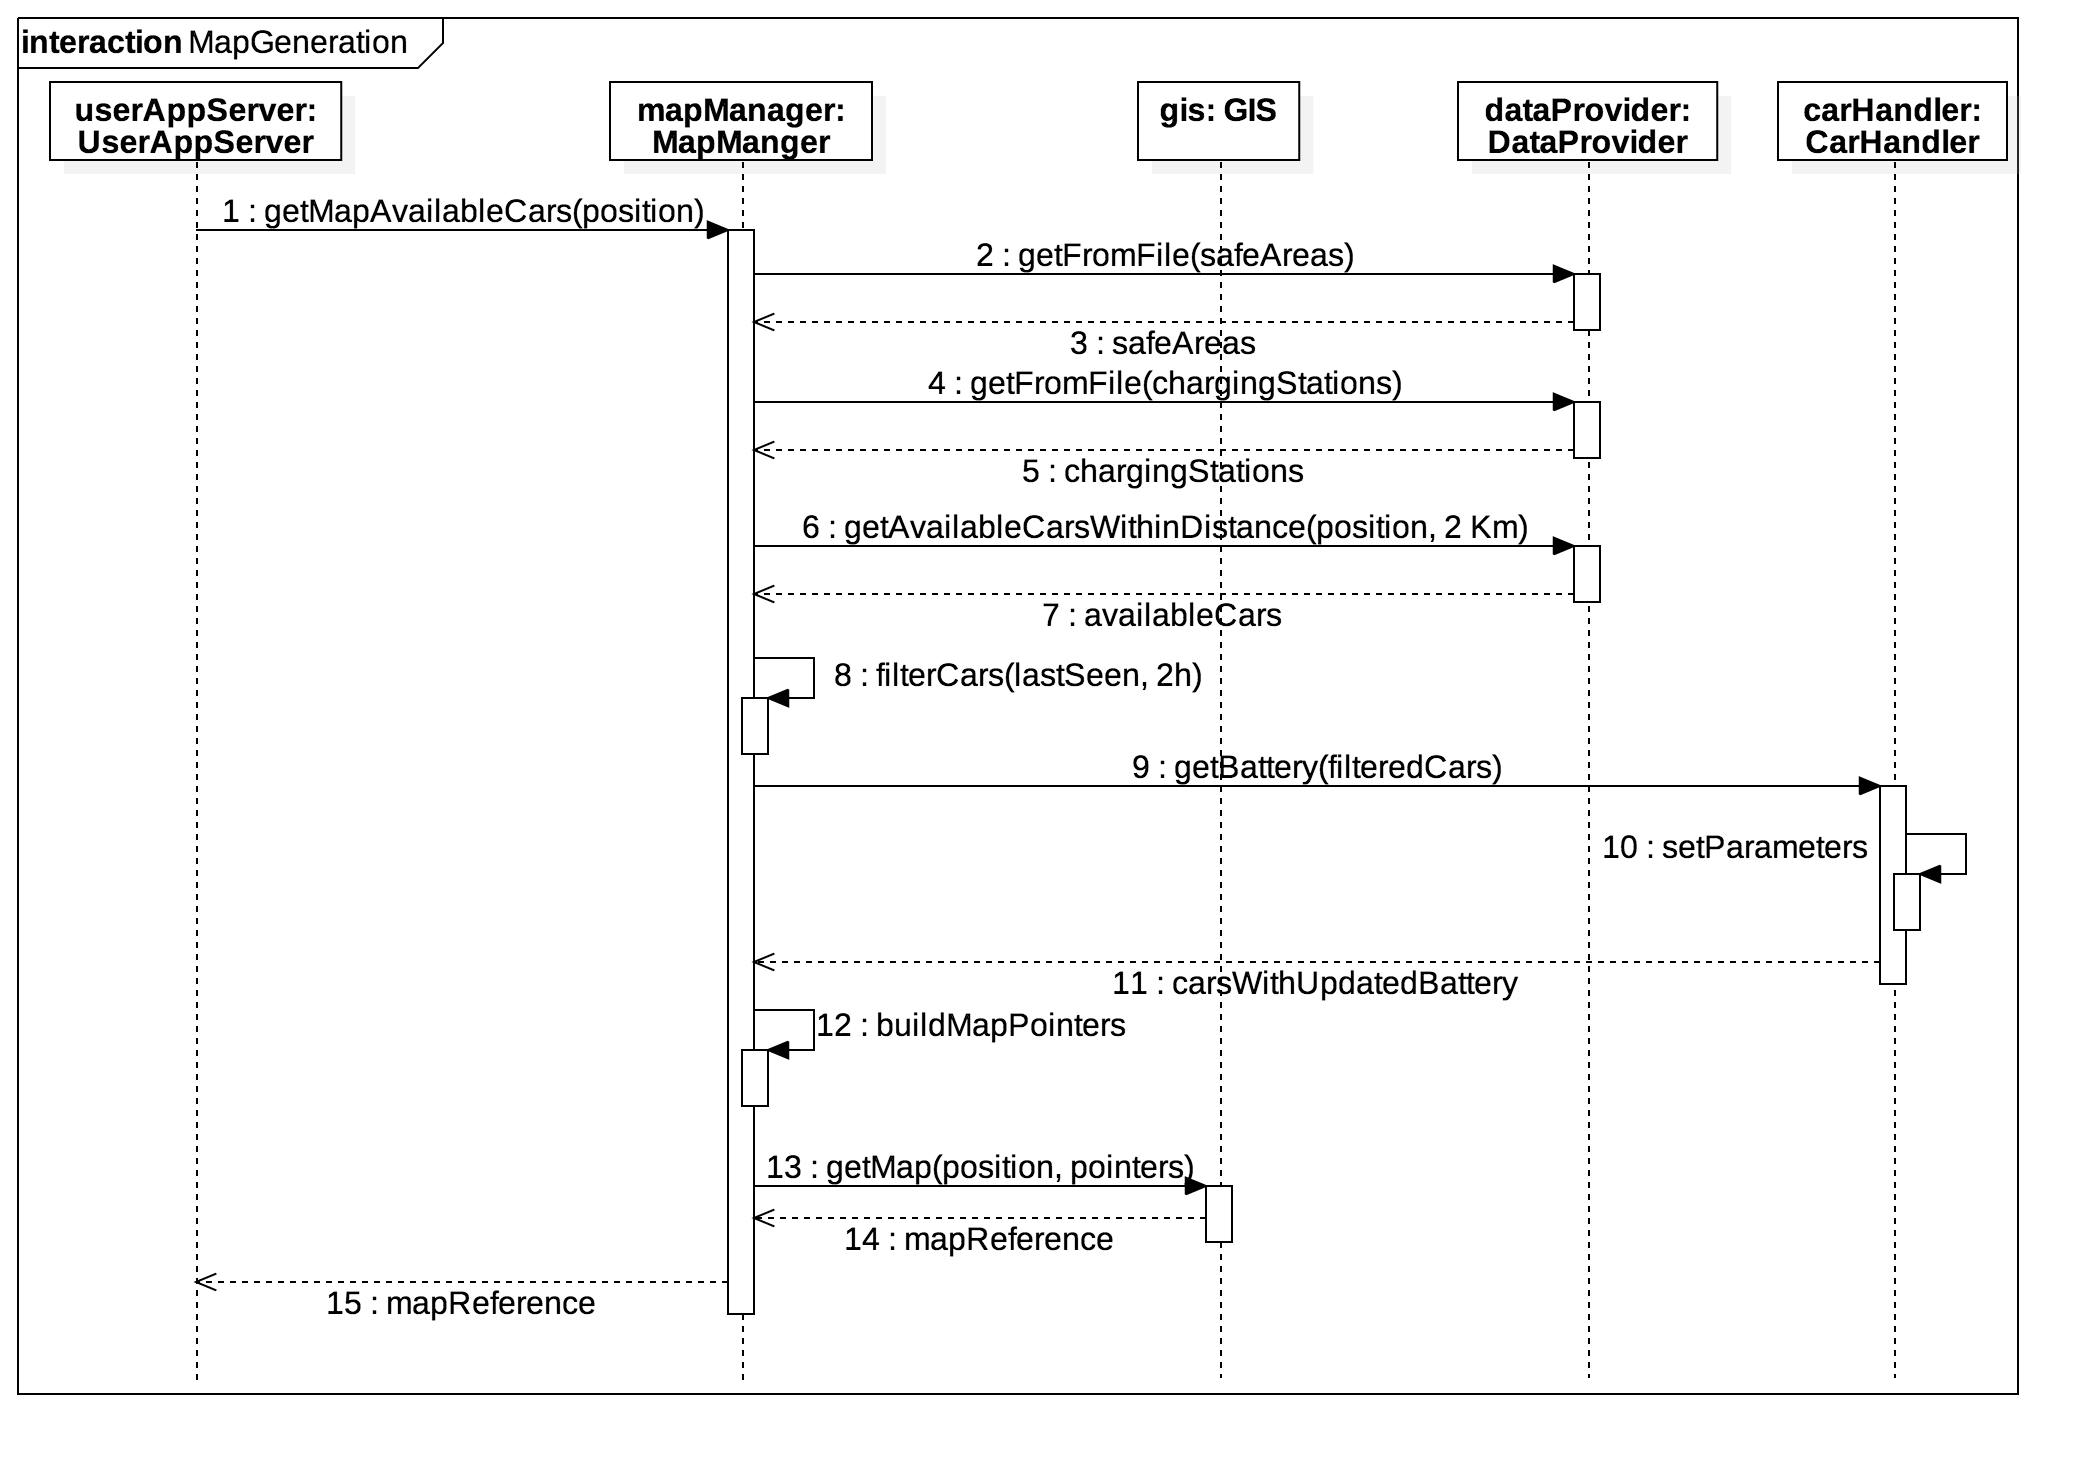
\includegraphics[angle=0,width=\linewidth]{sequenceDiagrams/MapGeneration}
	\caption{
		\label{fig:mapGeneration} 
		\emph{Map generation} sequence diagram
	}
\end{figure}

\clearpage
\subsubsection{Car reservation}
The diagram in \autoref{fig:sequenceCarReservation} shows the car reservation process.\\
The \mbox{\emph{MoneySavingOptionManager}} component determines the appropriate charging station for the money saving option given the user destination using the algorithm described in the \hyperref[sec:msoAlgorithm]{proper section}.

\paragraph{Interactions not represented}The \emph{ReservationRequestManager} need an interaction with the external GIS API in order to convert into latitude and longitude the destination inserted by the user for the money saving option.
\begin{figure}[h!]
	\centering
	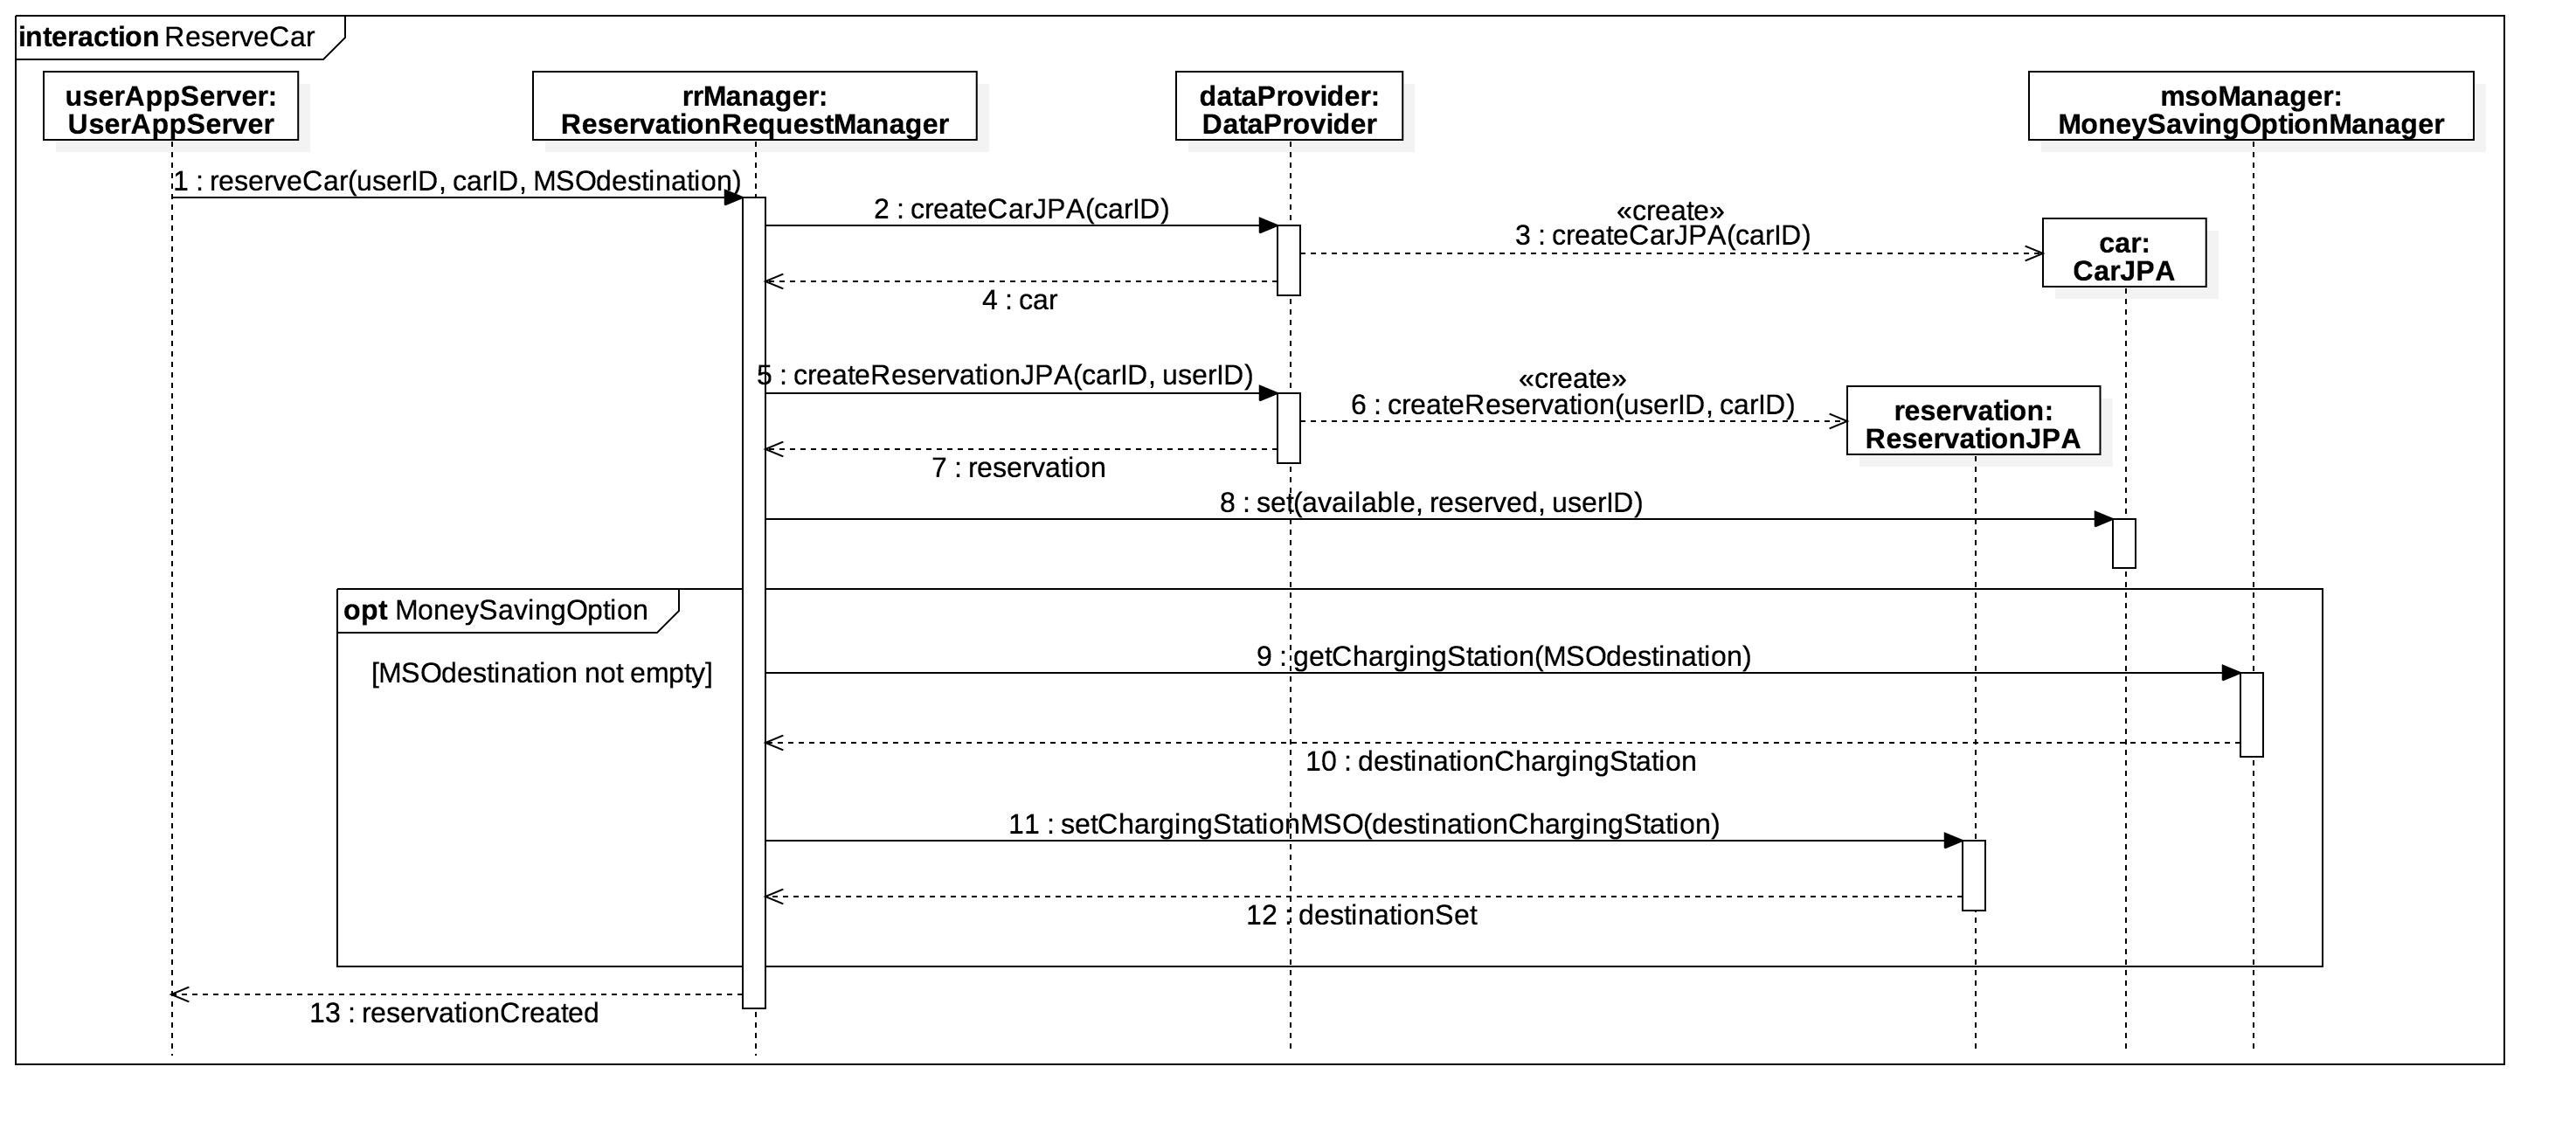
\includegraphics[angle=90,width=0.85\linewidth]{sequenceDiagrams/ReserveCar}
	\caption{
		\label{fig:sequenceCarReservation} 
		\emph{Car reservation} sequence diagram
	}
\end{figure}

\clearpage
\subsubsection{Performing a rent}
The following sequence diagrams show the interactions between the \mbox{Rent} \mbox{Manager} and other system components in different scenarios:
\begin{itemize}
	\item \autoref{fig:sequenceUnlockStartRent}: a user unlocks the car he reserved and starts the rent
	\item \autoref{fig:sequenceEndRent1}: a in use car notifies the system that the engine is off, there are no passengers in the car and the doors are closed
	\item \autoref{fig:sequenceEndRent2}: the rent just ended and the system initialize the payment procedure
\end{itemize}

\paragraph{Interactions not represented}
\begin{itemize}
	\item During the rent, at predetermined regular time intervals, \emph{CarUnlockManager} calls a primitive on the car through the \emph{CarHandler} component in order to retrieve the GPS position

	\item When an attribute is modified in a JPA object the changes are reflected into the \emph{DataProviderComponent} in order to keep the database updated
\end{itemize}
\clearpage

\begin{figure}[h!]
	\centering
	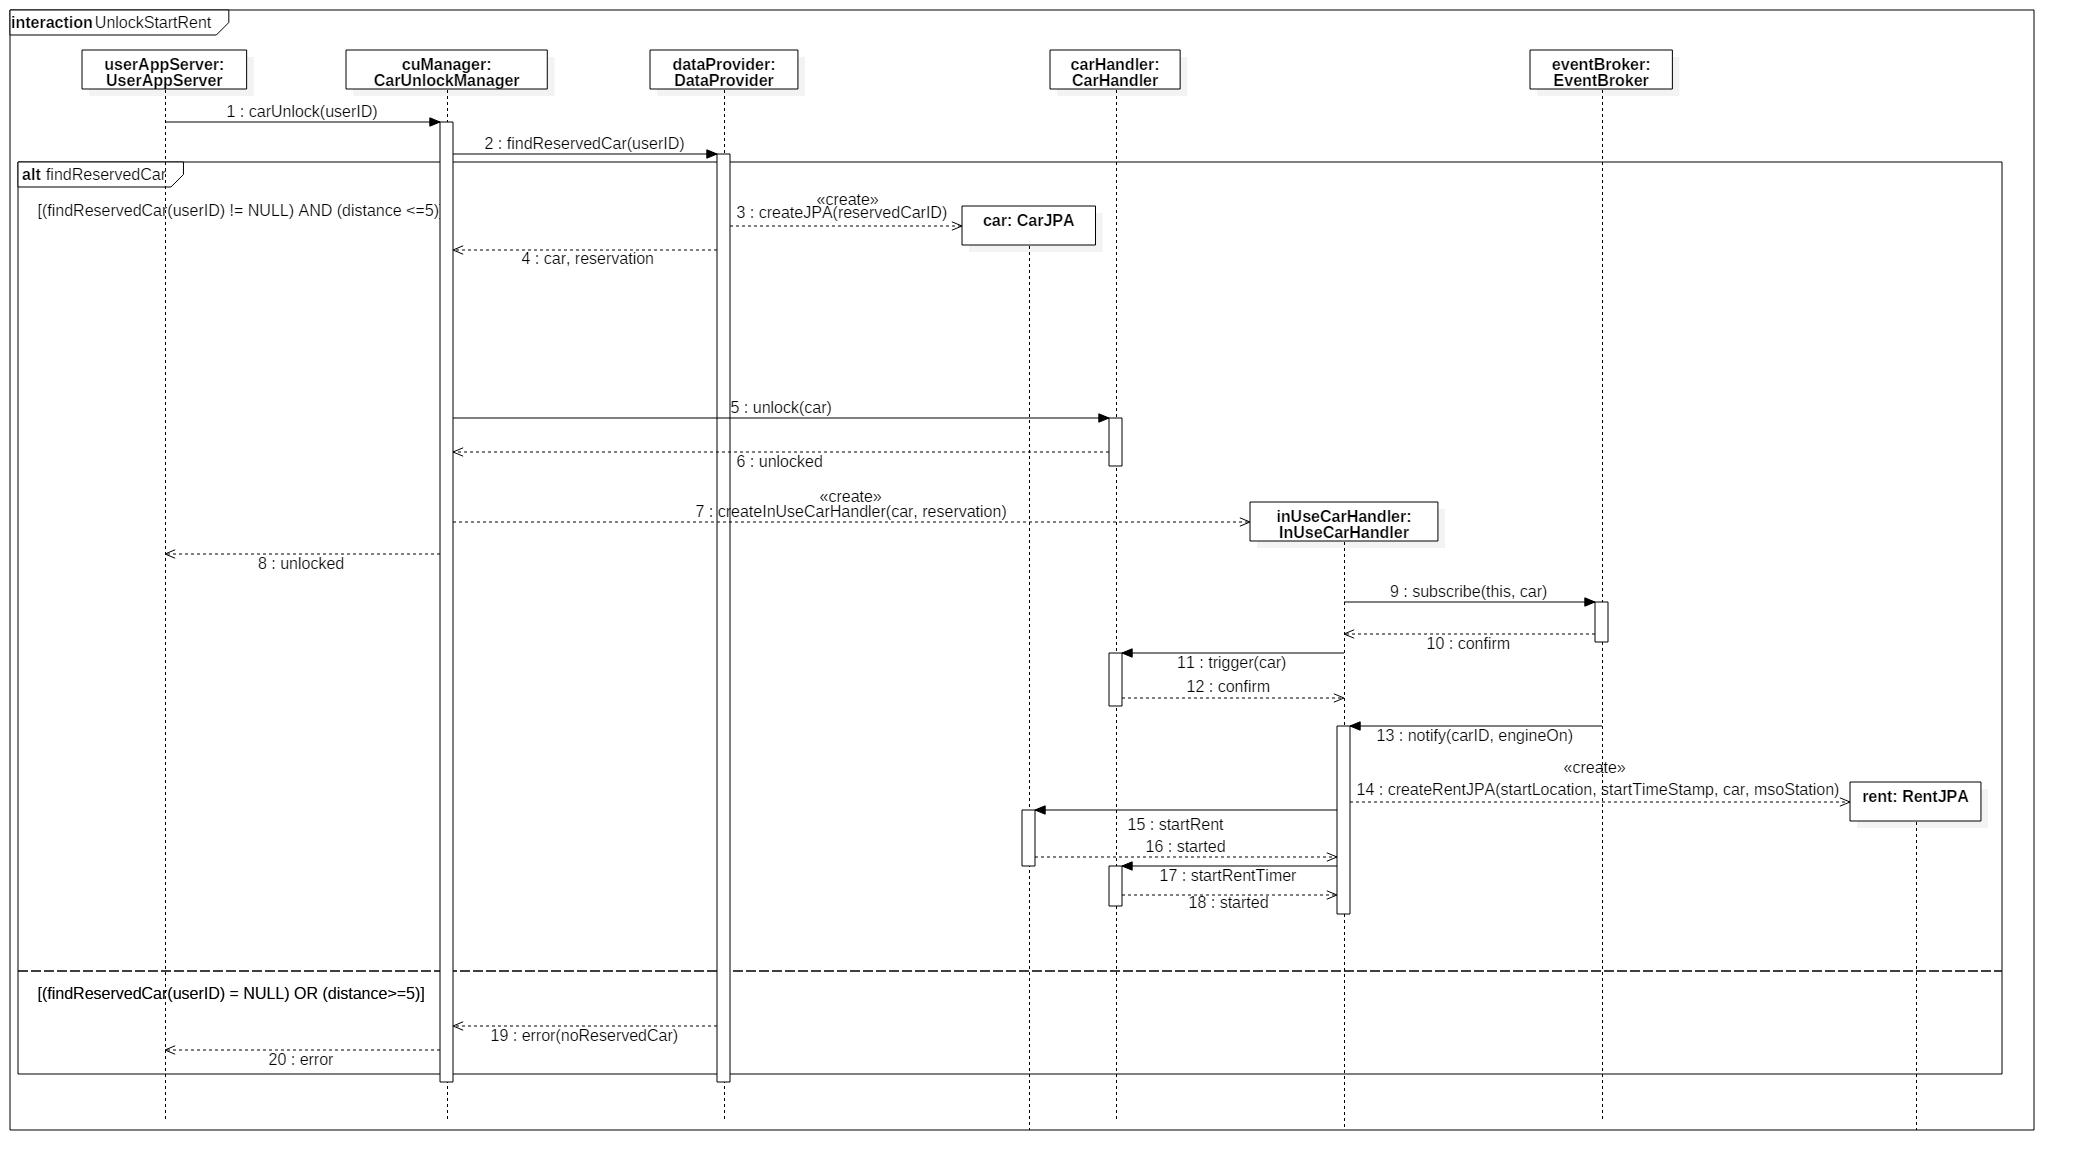
\includegraphics[angle=90,width=0.95\linewidth]{sequenceDiagrams/UnlockStartRent}
	\caption{
		\label{fig:sequenceUnlockStartRent} 
		\emph{Car unlock and start rent} sequence diagram
	}
\end{figure}
\begin{figure}[h!]
	\centering
	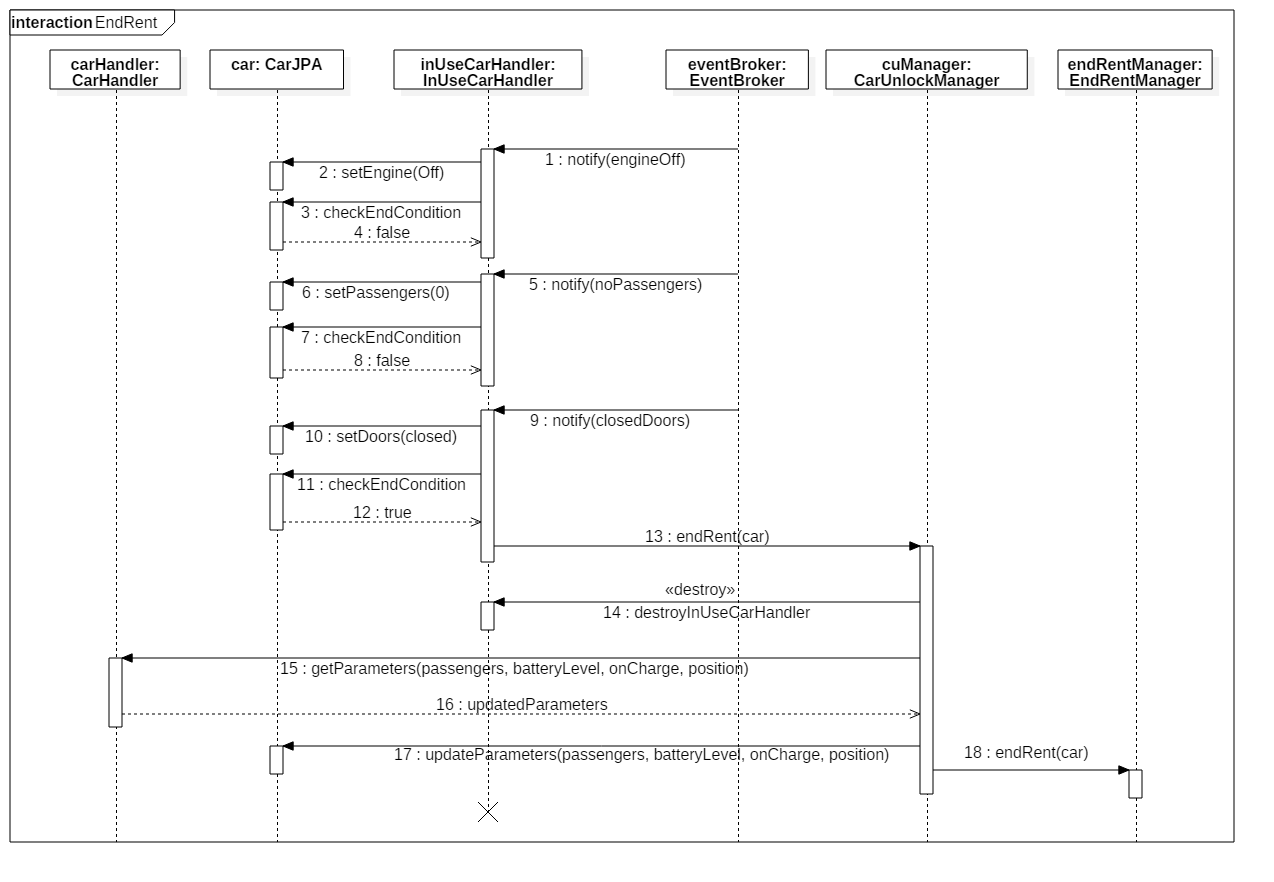
\includegraphics[angle=90,width=\linewidth]{sequenceDiagrams/EndRent}
	\caption{
		\label{fig:sequenceEndRent1} 
		\emph{End rent} sequence diagram (part 1)
	}
\end{figure}
\begin{figure}[h!]
	\centering
	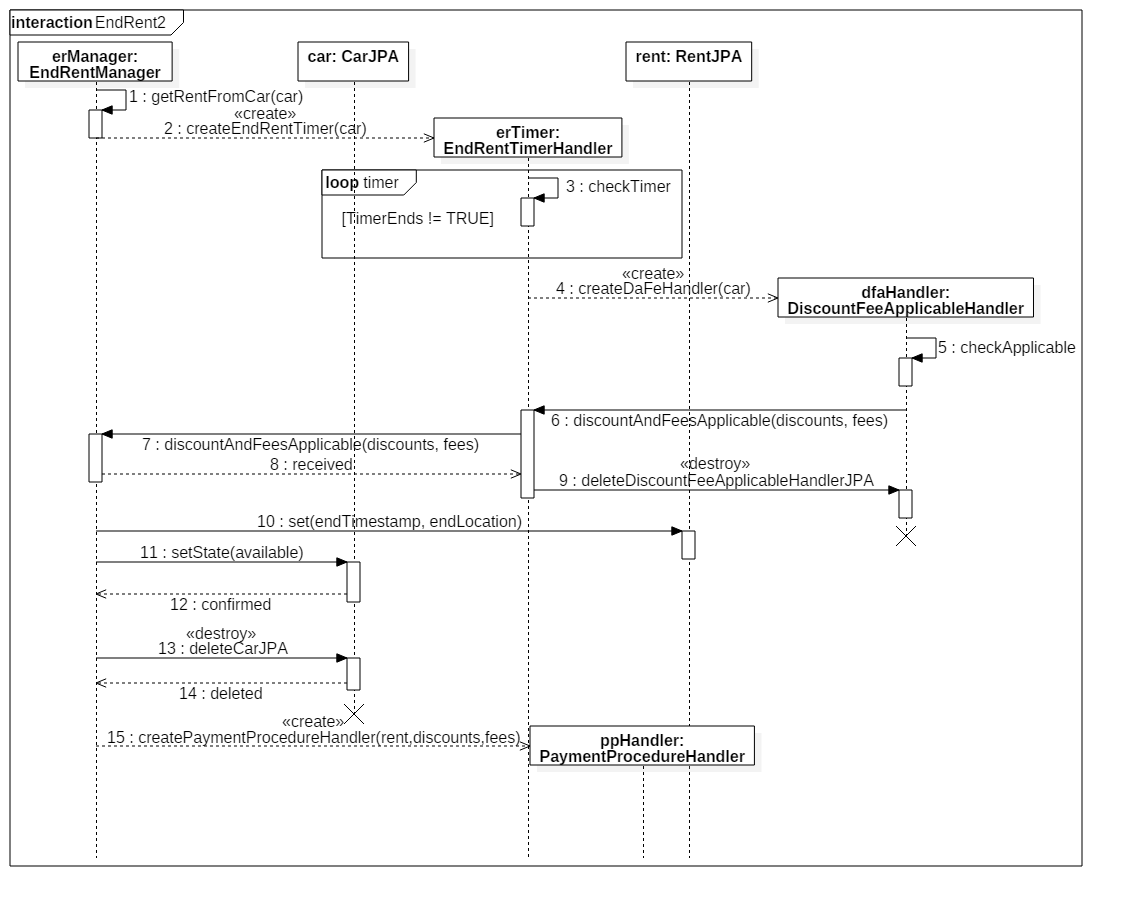
\includegraphics[angle=90,width=\linewidth]{sequenceDiagrams/EndRent2}
	\caption{
		\label{fig:sequenceEndRent2} 
		\emph{End rent} sequence diagram (part 2)
	}
\end{figure}

\clearpage
\subsubsection{Payment}
In the \autoref{fig:sequencePayment} is shown a rent payment initiated by the \emph{EndRentManager} component. This diagram is the continuation of the diagram in \autoref{fig:sequenceEndRent2}.

\paragraph{Interactions not represented} An interaction by the \emph{EndRentManager} with the \emph{DataProvider} component is required in order to ban a user if the payment is rejected.
\begin{figure}[h!]
	\centering
	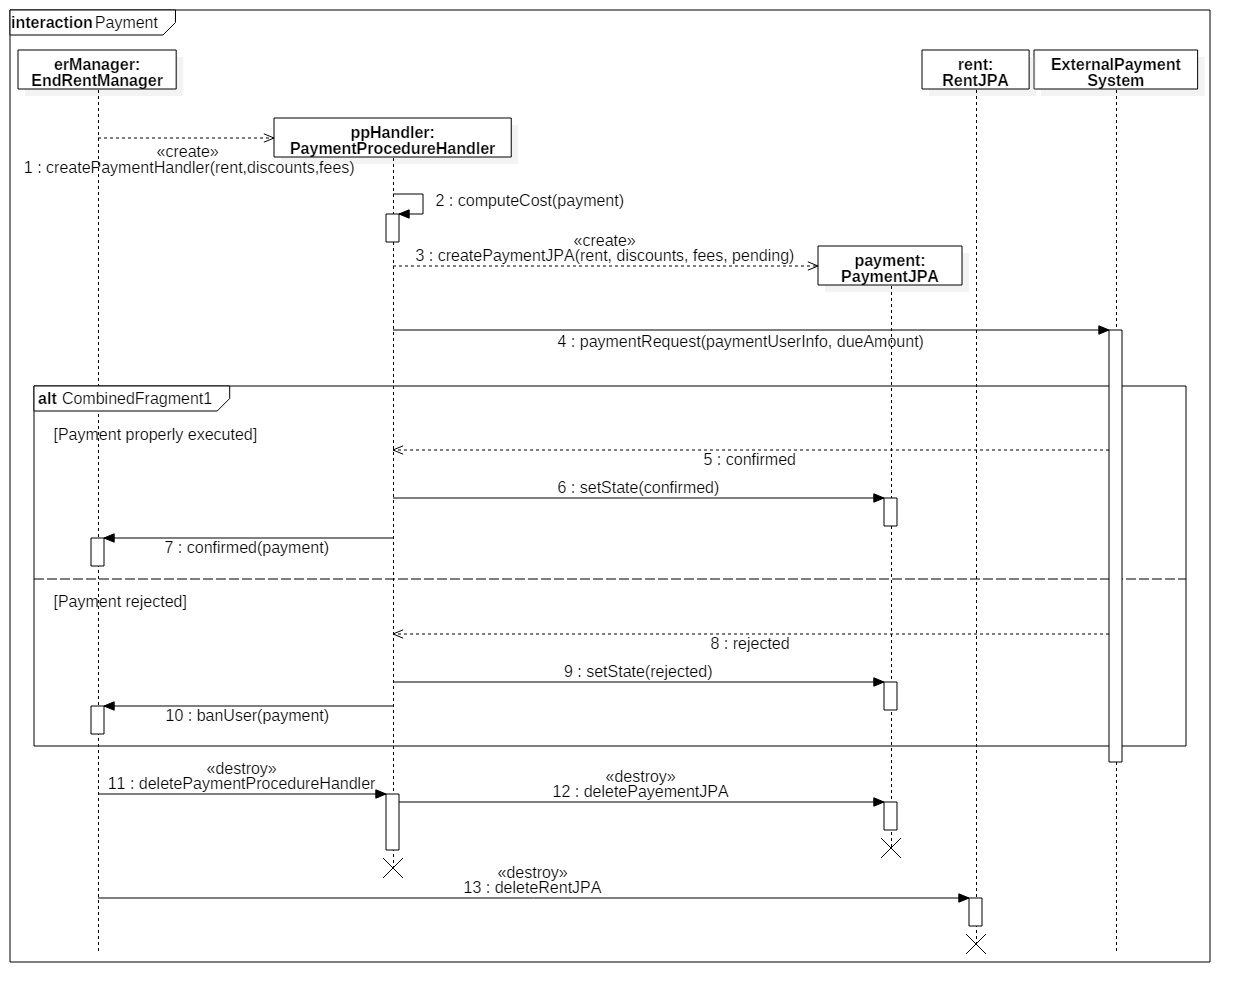
\includegraphics[angle=90,width=0.95\linewidth]{sequenceDiagrams/Payment}
	\caption{
		\label{fig:sequencePayment} 
		\emph{Payment} sequence diagram
	}
\end{figure}

\clearpage
\subsubsection{Reservation expiring}
To ensure a maximum reservation time of one hour, the \emph{ReservationTimer} component shown in \autoref{fig:sequenceReserveTimer} checks every minute the presence of expired reservations in the database. 

When a reservation expired is found, this component takes care of creating a payment request for the relative fee and deletes the reservation. 

\paragraph{Note}The extra time that could be granted to a reservation due to the timer interval and the system's latency is considered acceptable.

\paragraph{Interactions not represented} An interaction by the \emph{ReservationTimer} with the \emph{DataProvider} component is required in order to delete a reservation and to ban a user if the payment is rejected.
\begin{figure}[h!]
	\centering
	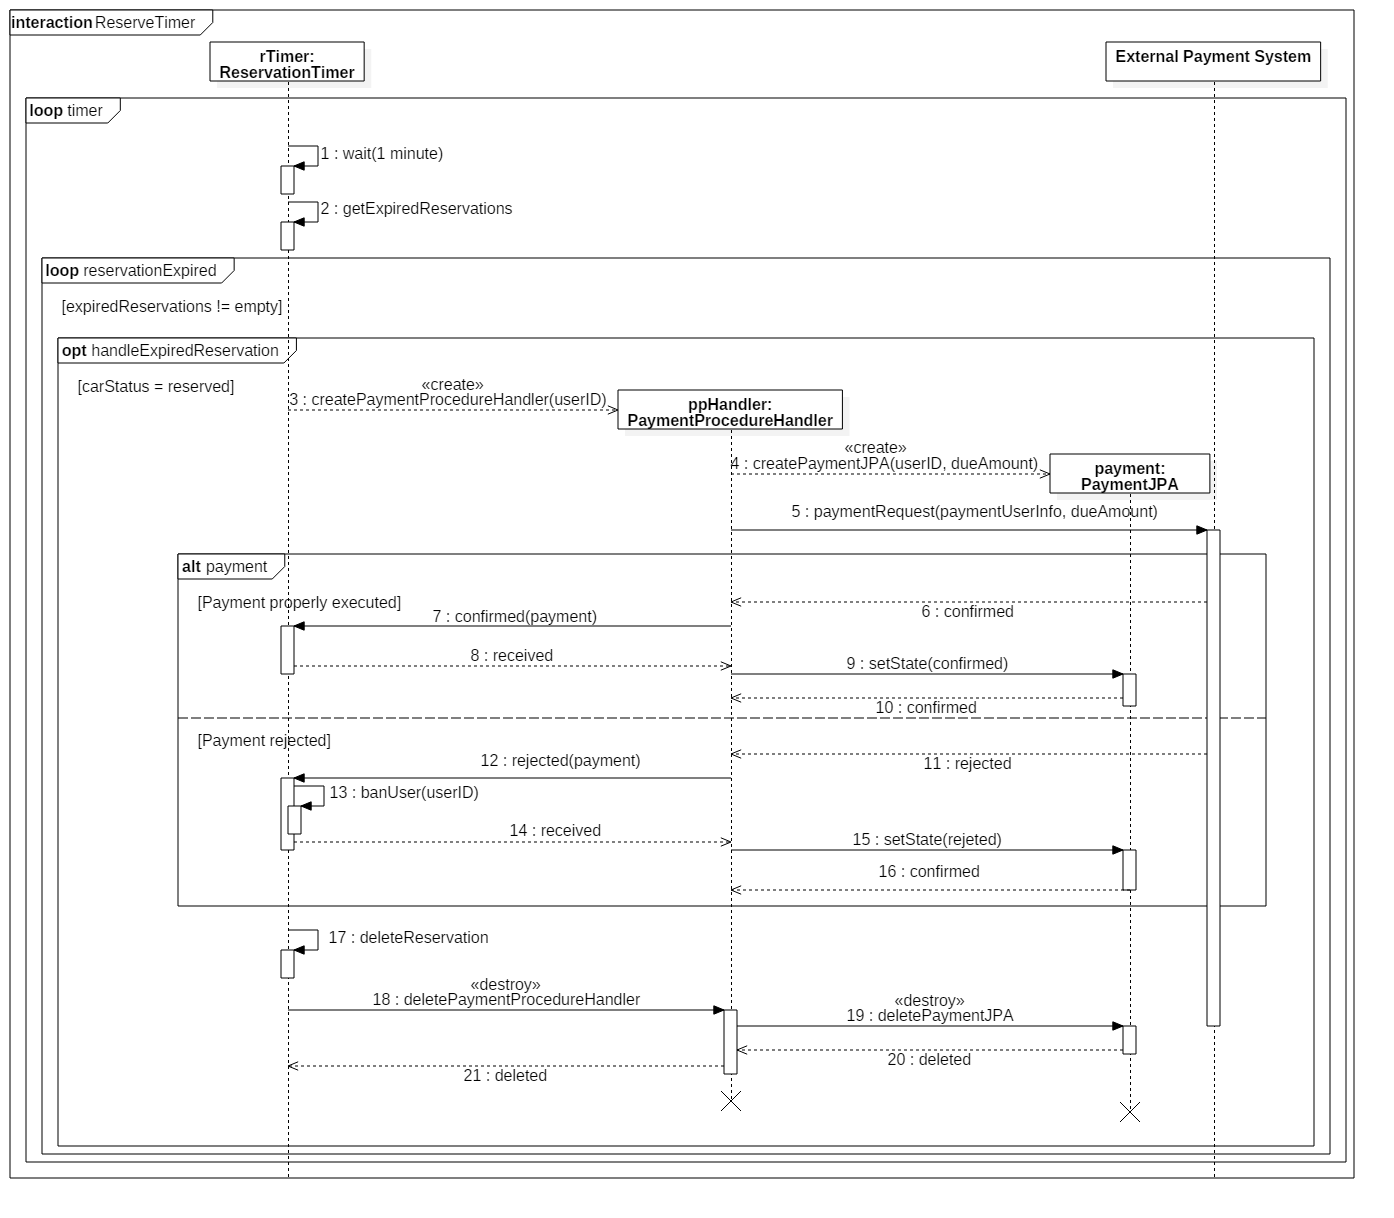
\includegraphics[angle=90,width=\linewidth]{sequenceDiagrams/ReserveTimer}
	\caption{
		\label{fig:sequenceReserveTimer} 
		\emph{Reservation expiring} sequence diagram
	}
\end{figure}

\clearpage
\subsubsection{Maintenance API and failures occurrence}
Our \emph{Maintenance API} is used by maintenance operators to obtain a list of car failures and to tag the cars back as Available when the failure has been fixed. The execution of these two commands is shown in \autoref{fig:sequenceMaintenanceAPI}.
\paragraph{Interactions not represented}When a car has to be tagged back as \mbox{Available} the \emph{MaintenanceDoneManager} takes care of verifying via \emph{DataProvider} and \emph{CarHandler} components if the car is associated with an open failure, if the doors are locked and all the others checks defined in the RASD.

\begin{figure}[h!]
	\centering
	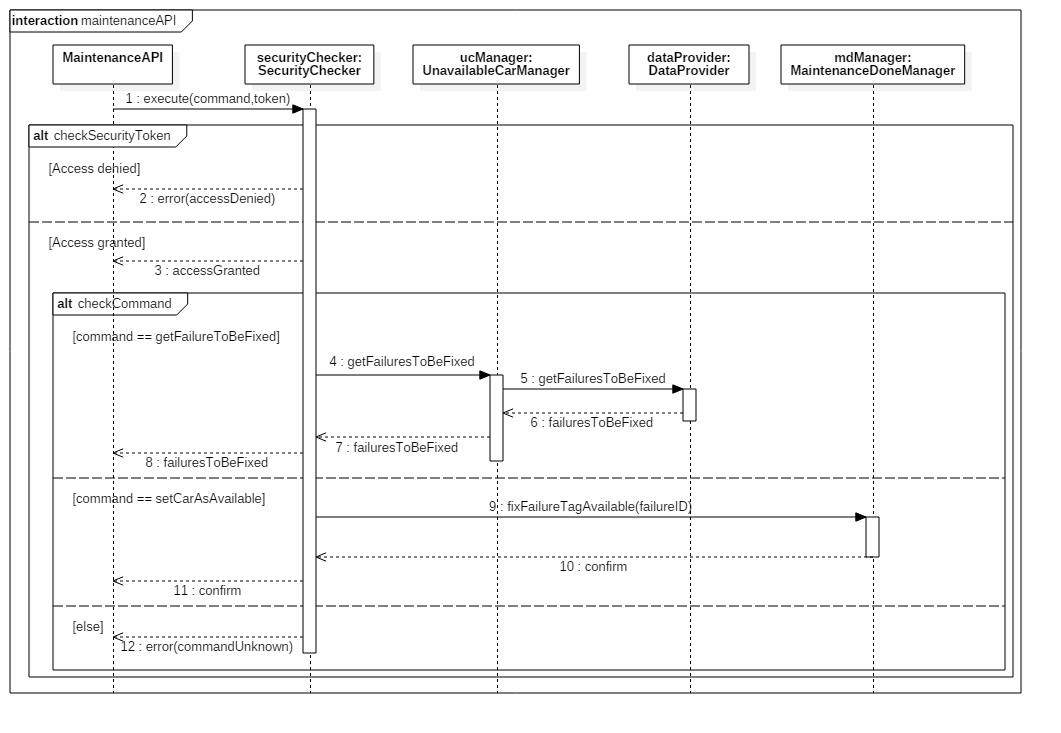
\includegraphics[angle=90,width=0.895\linewidth]{sequenceDiagrams/maintenanceAPI}
	\caption{
		\label{fig:sequenceMaintenanceAPI} 
		\emph{MaintenanceAPI} sequence diagram
	}
\end{figure}

\clearpage
\paragraph{Critical battery level}In \autoref{fig:sequenceMaintenanceBattery} is represented the case in which a car battery reaches its critical level.
\subparagraph{Note} The \emph{CarBatteryManager} component must be subscribed via the \mbox{\emph{EventBroker}} component to all cars and it must enable via the \emph{CarHandler} component the trigger for the critical battery level event. We can suppose that these operations are done during the initialization phase.
\begin{figure}[h!]
	\centering
	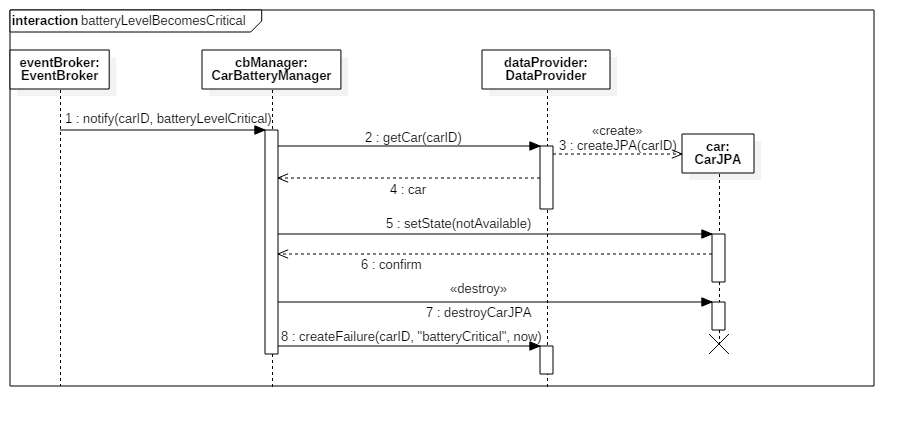
\includegraphics[width=\linewidth]{sequenceDiagrams/maintenanceBatteryLevel}
	\caption{
		\label{fig:sequenceMaintenanceBattery} 
		\emph{Battery level critical trigger} sequence diagram
	}
\end{figure}

\clearpage
\subsection{Component interfaces}

\subsubsection{Car-server interfaces}
All cars are provided with a module that grants TCP/IP connectivity over a dedicated subnet offered by a specific ISP. In order to ensure better security for the communications, in the same subnet is also located the server with the \mbox{\emph{CarEventHandler}} interface and the API used by Maintenance.

The \emph{CarHandler} component communicates to cars via the \mbox{\emph{CarPrimitives}} external API (using the JAX-RS API) which executes functions directly on car modules using a dedicated built-in connection.

\subsubsection{Maintenance API interface}
The Maintenance API must be realized using the REST paradigm. The external maintenance system should query the Maintenance API at predefined time intervals in order to retrieve an updated list of car failures paired with proper software keys in order to unlock the doors.

Considering the importance of the operations performed, these security measures must be taken into consideration:
\begin{itemize}
	\item The API must be accessible only over the system dedicated subnet
	\item A security token must be provided in order to perform any action through the API
\end{itemize}
The maintenance operators have been provided a smartphone which is connected in the same dedicated subnet used for cars and for the server with the Maintenance API.
Security tokens must be negotiated by our system and the external maintenance service.

\subsubsection{User Application interface}
The \emph{UserAppIntF} interface is responsible for communications between the user application and the user application server.

Because of the nature of exchanged data (credit card number, password, and privacy-related information), the protocol to be used is HTTPS.

\subsubsection{Customer Care interface}
Via the \emph{CustomerCareIntF} interface is responsible for communications between the customer care application and the CustomerCare server.

All computers used by the customer care service are connected in the same dedicated subnet as the CustomerCare server and this web server is accessible only from the aforementioned subnet. 

A VPN is used to achieve what mentioned above. Because of corporate data exchange, the protocol to be used id HTTPS

\subsubsection{GIS API}
Using this external API of a \emph{Geographical Information System} our system is able to:
\begin{itemize}
	\item retrieve an updated map centered on a given position
	\item get the latitude and longitude of a given location and vice versa
\end{itemize}

\subsubsection{DBMS API}
Trough the DBMS API the system can retrieve and write data into the database. Note that the \mbox{\emph{DataProvider}} component is the only one that access directly this interface.

\subsubsection{Payments API}
Payment transactions are processed using this external API of a \emph{Web based electronic payment system}.\\
Information required from this API are in order to complete a payment transaction (fetched from the database):
\begin{itemize}
	\item name and surname of the payer
	\item due amount
	\item credit card number
\end{itemize}
Data encryption must be taken into consideration.\\
The API response must be the payment outcome in JSON format (succeded or rejected).
\subsection{Architectural style and patterns}
\subsection{Other design decision}
